% ***************************************************
% A Classic Thesis Style
% An Homage to The Elements of Typographic Style
%
% Copyright (C) 2012 Andr\'e Miede http://www.miede.de
%
% If you like the style then I would appreciate a postcard. My
% address can be found in the file ClassicThesis.pdf. A collection
% of the postcards I received so far is available online at 
% http://postcards.miede.de
%
% License:
% This program is free software; you can redistribute it and/or
% modify it under the terms of the GNU General Public License as
% published by the Free Software Foundation; either version 2 of
% the License, or (at your option) any later version.
%
% This program is distributed in the hope that it will be useful,
% but WITHOUT ANY WARRANTY; without even the implied warranty of
% MERCHANTABILITY or FITNESS FOR A PARTICULAR PURPOSE.  See the
% GNU General Public License for more details.
%
% You should have received a copy of the GNU General Public
% License along with this program; see the file COPYING.  If not,
% write to the Free Software Foundation, Inc., 59 Temple Place -
% Suite 330, Boston, MA 02111-1307, USA.
%
% ***************************************************************
% Note:
%    * You must not use "u etc. in strings/commands that will be spaced out (use \"u or real umlauts instead)
%    * New enumeration (small caps): \begin{aenumerate} \end{aenumerate}
%    * For margin notes: \marginpar or \graffito{}
%    * Do not use bold fonts in this style, it is designed around them
%    * Use tables as in the examples
%    * See classicthesis-preamble.sty for useful commands
% ****************************************************************

\documentclass[ twoside, 
			openright,
			% letterpaper a4paper
			titlepage, 
			numbers=noenddot,
			headinclude, %1headlines
            		footinclude=true, 
			cleardoublepage=empty,
			abstractoff, % <--- obsolete, remove (todo)
			BCOR=5mm,
			paper=a4, 
			fontsize=11pt, %11pt,
			]{scrreprt}

%*****************************************************************
% Note: Make all your adjustments in here
%*****************************************************************

% \usepackage[backref, backend=biber]{biblatex}
\usepackage[backref,
		backend=bibtex,
            	maxbibnames=99,
            	natbib=true,
            	firstinits=false,
            	style=authoryear-comp,
            	sortcites=false,
            	doi=false,
            	url=false]{biblatex}
\bibliography{Bibliography}	

% ****************************************************************
% classicthesis-config.tex 
% formerly known as loadpackages.sty, classicthesis-ldpkg.sty, and
% classicthesis-preamble.sty Use it at the beginning of your
% ClassicThesis.tex, or as a LaTeX Preamble in your
% ClassicThesis.{tex,lyx} with % ****************************************************************
% classicthesis-config.tex 
% formerly known as loadpackages.sty, classicthesis-ldpkg.sty, and
% classicthesis-preamble.sty Use it at the beginning of your
% ClassicThesis.tex, or as a LaTeX Preamble in your
% ClassicThesis.{tex,lyx} with % ****************************************************************
% classicthesis-config.tex 
% formerly known as loadpackages.sty, classicthesis-ldpkg.sty, and
% classicthesis-preamble.sty Use it at the beginning of your
% ClassicThesis.tex, or as a LaTeX Preamble in your
% ClassicThesis.{tex,lyx} with \input{classicthesis-config}
% ****************************************************************
% If you like the classicthesis, then I would appreciate a
% postcard. My address can be found in the file
% ClassicThesis.pdf. A collection of the postcards I received so
% far is available online at http://postcards.miede.de
% ****************************************************************

% ****************************************************************
% 1. Configure classicthesis for your needs here, e.g., remove
% "drafting" below in order to deactivate the time-stamp on the
% pages
% ****************************************************************
\PassOptionsToPackage{eulerchapternumbers,
					listings,
					%drafting,
				 	pdfspacing,
					floatperchapter,
					%linedheaders,
				 	subfig,
					beramono,
					eulermath,
					parts}{classicthesis}										

% ****************************************************************
% Triggers for this config
% **************************************************************** 
\usepackage{ifthen}
\newboolean{enable-backrefs} % enable backrefs in the bibliography
\setboolean{enable-backrefs}{false} % true false
% TODO backref is incompatible?
% ****************************************************************
%*********************************************************************************
% 2.a Math
%*********************************************************************************
\PassOptionsToPackage{fleqn}{amsmath} % math environments and more by the AMS 
\usepackage{amsmath,amssymb}

\usepackage{amsthm}
\usepackage{amssymb}
\renewcommand\qedsymbol{$\blacksquare$}

\theoremstyle{definition}
\newtheorem{definition}{Definition}[chapter]
\newtheorem{theorem}{Theorem}[chapter]

\theoremstyle{plain}
\newtheorem{observation}[definition]{Observation}
\newtheorem{corollary}[theorem]{Corollary}
\newtheorem{lemma}[theorem]{Lemma}
\newtheorem{assumption}[theorem]{Assumption}
% **********************************************************************



% ****************************************************************
% 3. Personal data and user ad-hoc commands
% ****************************************************************
\newcommand{\myTitle}{Stochastic Variance Reduced Policy Gradient\xspace}
\newcommand{\myTitleIT}{Stochastic Variance Reduced Policy Gradient \xspace}
\newcommand{\myFirstAuthorName}{Damiano Binaghi\xspace}
\newcommand{\myMatrFirstAuthor}{858458\xspace}
\newcommand{\mySecondAuthorName}{Giuseppe Canonaco\xspace}
\newcommand{\myMatrSecondAuthor}{852749\xspace}
\newcommand{\mySupervisor}{Marcello Restelli\xspace} % relatore
\newcommand{\myOtherSupervisor}{Matteo Papini\xspace} % co relatori
\newcommand{\myOtherOtherSupervisor}{Matteo Pirotta\xspace}
\newcommand{\myCoExaminer}{\xspace} % contro-relatore
\newcommand{\myFaculty}{Facolt\`a di Ingegneria\xspace}
\newcommand{\mySchool}{Scuola di Ingegneria Industriale e dell\textquotesingle Informazione\xspace}
\newcommand{\myDepartment}{Dipartimento di Elettronica, Informazione e Bioingegneria\xspace}
\newcommand{\myCourseFirstPart}{Master of Science in\xspace}
\newcommand{\myCourseFirstPartIT}{Corso di Laurea Magistrale in\xspace}
\newcommand{\myCourseSecondPart}{Computer Science and Engineering\xspace}
\newcommand{\myCourseSecondPartIT}{Ingegneria Informatica\xspace}
\newcommand{\myUni}{Politecnico di Milano\xspace}
\newcommand{\myLocation}{Milan\xspace}
\newcommand{\myTime}{April 2018\xspace}
\newcommand{\myVersion}{version 1.0\xspace}
\newcommand{\myAcademicYear}{Academic Year 2017-2018\xspace}
\newcommand{\myAcademicYearIT}{Anno Accademico 2017-2018\xspace}




% ********************************************************************
% Setup, fine tuning, and useful commands
% ********************************************************************
\newcounter{dummy} % necessary for correct hyperlinks (to index, bib, etc.)
\newlength{\abcd} % for ab..z string length calculation
\providecommand{\mLyX}{L\kern-.1667em\lower.25em\hbox{Y}\kern-.125emX\@}
% from here till the end of the section, you can modify whatever you want
\newcommand{\ie}{i.\,e.\ }
\newcommand{\Ie}{I.\,e.\ }
\newcommand{\eg}{e.\,g.\ }
\newcommand{\Eg}{E.\,g.\ }
% referencing commands
\newcommand{\myEq}[1]{equation \eqref{#1}}
\newcommand{\MyEq}[1]{Equation \eqref{#1}}
\newcommand{\myFig}[1]{figure \ref{#1}}
\newcommand{\MyFig}[1]{Figure \ref{#1}}
\newcommand{\myTab}[1]{table \ref{#1}}
\newcommand{\MyTab}[1]{Table \ref{#1}}
\newcommand{\mySubsec}[1]{subsection \ref{#1}}
\newcommand{\MySubsec}[1]{Subsection \ref{#1}}
\newcommand{\mySec}[1]{section \ref{#1}}
\newcommand{\MySec}[1]{Section \ref{#1}}
\newcommand{\myChap}[1]{chapter \ref{#1}}
\newcommand{\MyChap}[1]{Chapter \ref{#1}}
\newcommand{\myAppendix}[1]{appendix \ref{#1}}
\newcommand{\MyAppendix}[1]{Appendix \ref{#1}}
\newcommand{\myEmph}[1]{\textsc{#1}}

% **********************************************************************
%%%CUSTOM COMMANDS%%%
%***********************************************************************
%Math
\newcommand{\realspace}{\mathbb R}      % realspace
\newcommand{\transpose}[1]{{#1}^\texttt{T}}
\DeclareMathOperator*{\argmax}{arg\,max}
\DeclareMathOperator*{\argmin}{arg\,min}
\DeclareMathOperator*{\EV}{\mathbb{E}}
\DeclareMathOperator{\Tr}{Tr}
\DeclareMathOperator*{\Cov}{\mathbb{C}ov}
\DeclareMathOperator*{\Var}{\mathbb{V}ar}
\newcommand{\EVV}[2][\ppvect \in \ppspace]{\EV_{#1}\left[{#2}\right]}
\newcommand{\norm}[2][\infty]{\left\|#2\right\|_{#1}}
\newcommand{\Dij}[2]{\frac{\partial^{2}{#1}}{\partial{#2}_i\partial{#2}_j}}
\newcommand{\de}{\,\mathrm{d}}
\newcommand{\dotprod}[2]{\left\langle#1,#2\right\rangle}
\newcommand{\dnabla}{\nabla\!\!\!\!\nabla}
%RL
\newcommand{\vtheta}{\boldsymbol{\theta}}
\newcommand{\Aspace}{\mathcal{A}}
\newcommand{\Sspace}{\mathcal{S}}
\newcommand{\Tspace}{\mathcal{T}}
\newcommand{\Transition}{\mathcal{P}}
\newcommand{\Reward}{\mathcal{R}}
\newcommand{\stationary}{d_{\rho}^{\pi_{\vtheta}}(s)}
\newcommand{\policy}{\pi_{\vtheta}(a \vert s)}
\newcommand{\pol}{\pi_{\vtheta}}
\newcommand{\trajdistr}{\pi_{\vtheta}(\tau)}
\newcommand{\score}[2]{\nabla\log p_{#1}(#2)}
\newcommand{\Qfun}{Q^{\pi_{\vtheta}}(s,a)}
\newcommand{\Vfun}{V^{\pi_{\vtheta}}(s)}
\newcommand{\vTheta}{\boldsymbol{\Theta}}
\newcommand{\vphi}{\boldsymbol{\phi}}
\newcommand{\gradJ}[1]{\nabla J(#1)}
\newcommand{\gradApp}[2]{\widehat{\nabla}_{#2}J(#1)}
\newcommand{\eqdef}{\mathrel{\mathop:}=}
\newcommand{\Dataset}{\mathcal{D}}
%Specific
\newcommand{\Ets}[2][t]{\mathbb{E}_{#1\vert s}\left[#2\right]}
\newcommand{\Es}[1]{\mathbb{E}_{s}\left[#1\right]}
\newcommand{\Covts}[3][t]{{\mathbb{C}\text{ov}}_{#1\vert s}\left(#2,#3\right)}
\newcommand{\Covs}[2]{{\mathbb{C}\text{ov}}_{s}\left(#1,#2\right)}
\newcommand{\Varts}[2][t]{{\mathbb{V}\text{ar}}_{#1\vert s}\left[#2\right]}
\newcommand{\Vars}[1]{{\mathbb{V}\text{ar}}_{s}\left[#1\right]}
\newcommand{\gradBlack}[1]{\blacktriangledown J(#1)}
\newcommand{\gradIdeal}[1]{\dnabla J(#1)}
\newcommand{\VARRF}{V}
\newcommand{\GRADLOG}{G}
\newcommand{\VARIS}{W}
\newcommand{\HESSLOG}{F}
% short forms 
\newcommand{\wt}[1]{\widetilde{#1}}
\newcommand{\wh}[1]{\widehat{#1}}
\newcommand{\wo}[1]{\overline{#1}}
\newcommand{\wb}[1]{\overline{#1}}
%%%%%%


% **********************************************************************
% 3. Loading some handy packages
% **********************************************************************
\PassOptionsToPackage{fleqn}{amsmath} % math environments and more by the AMS 
\usepackage{amsmath}
\usepackage{algorithm}
\usepackage{algorithmic}
\usepackage{amsthm}
\usepackage{amssymb}
\usepackage{geometry}
\renewcommand\qedsymbol{$\blacksquare$}		

\PassOptionsToPackage{autostyle,italian=guillemets,threshold=2}{csquotes}
 	\usepackage{csquotes}

\PassOptionsToPackage{american,italian}{babel}
	 \usepackage{babel}

 \usepackage{textcomp} % fix warning with missing font shapes
\usepackage{scrhack} % fix warnings when using KOMA with listings package          
\usepackage{xspace} % to get the spacing after macros right  
\usepackage{mparhack} % get marginpar right
\usepackage{fixltx2e} % fixes some LaTeX stuff
\usepackage{microtype}
\usepackage[normalem]{ulem} % to have strikethrough text

\PassOptionsToPackage{printonlyused,smaller}{acronym}
	\usepackage{acronym} % nice macros for handling all acronyms in the thesis
% **********************************************************************
% Recommended, but optional, packages for figures and better typesetting:
\usepackage{microtype}
\usepackage{graphicx}
\graphicspath{ {images/} }


\usepackage{microtype}
\usepackage{graphicx}
\graphicspath{ {images/} }
%\usepackage{subfigure}
\usepackage{booktabs} % for professional tables

% hyperref makes hyperlinks in the resulting PDF.
% If your build breaks (sometimes temporarily if a hyperlink spans a page)
% please comment out the following usepackage line and replace
% \usepackage{icml2018} with \usepackage[nohyperref]{icml2018} above.
\usepackage{hyperref}
%%%USEFUL PACKAGES%%%
\usepackage{nicefrac}       % compact symbols for 1/2, etc.
\usepackage{mathtools}
\usepackage{pifont}
\usepackage[makeroom]{cancel}
\usepackage{placeins}

%e.g. ...
\usepackage{xspace}
\DeclareRobustCommand{\eg}{e.g.,\@\xspace}
\DeclareRobustCommand{\ie}{i.e.,\@\xspace}
\DeclareRobustCommand{\wrt}{w.r.t.\@\xspace}



% **********************************************************************
% 4. Setup floats: tables, (sub)figures, and captions
% **********************************************************************
\usepackage{tabularx} % better tables
	\setlength{\extrarowheight}{3pt} % increase table row height
\newcommand{\tableheadline}[2]{\multicolumn{1}{#1}{\normalsize\spacedlowsmallcaps{#2}}}
\newcommand{\tableheadlineMore}[3]{\multicolumn{#1}{#2}{\normalsize\spacedlowsmallcaps{#3}}}
\newcommand{\tablefirstcol}[2]{\multicolumn{1}{#1}{\textbf{#2}}}

\usepackage{caption}
	\captionsetup{format=hang,labelfont={sf,bf},font=small}
\usepackage{colortbl}
\usepackage{multirow}

\usepackage{subfig}
\usepackage{siunitx}
% *********************************************************************


% *********************************************************************
% 5. Setup code listings
% *********************************************************************
\usepackage{listings}
\lstloadlanguages{bash, C++, Java, Matlab}

% for special keywords
\lstset{language=[LaTeX]Tex,
    keywordstyle=\color{RoyalBlue},%\bfseries,
    basicstyle=\small\ttfamily,
    %identifierstyle=\color{NavyBlue},
    commentstyle=\color{Green}\ttfamily,
    stringstyle=\rmfamily,
    numbers=none,%left,%
    numberstyle=\scriptsize,%\tiny
    stepnumber=5,
    numbersep=8pt,
    showstringspaces=false,
    breaklines=true,
    frameround=ftff,
    frame=single,
    belowcaptionskip=.75\baselineskip
    %frame=L
} 
% *********************************************************************


% *********************************************************************
% 6. PDFLaTeX, hyperreferences and citation backreferences
% *********************************************************************
% ********************************************************************
% Using PDFLaTeX
% ********************************************************************
\PassOptionsToPackage{pdftex,hyperfootnotes=false,pdfpagelabels}{hyperref}
	\usepackage{hyperref}  % backref linktocpage pagebackref
\pdfcompresslevel=9
\pdfadjustspacing=1 
\PassOptionsToPackage{pdftex}{graphicx}
	\usepackage{graphicx} 

% ********************************************************************
% Setup the style of the backrefs from the bibliography
% (translate the options to any language you use)
% ********************************************************************
\newcommand{\backrefnotcitedstring}{\relax}%(Not cited.)
\newcommand{\backrefcitedsinglestring}[1]{(Cited on page~#1.)}
\newcommand{\backrefcitedmultistring}[1]{(Cited on pages~#1.)}
\ifthenelse{\boolean{enable-backrefs}}%
{%
		\PassOptionsToPackage{hyperpageref}{backref}
		\usepackage{backref} % to be loaded after hyperref package 
		   \renewcommand{\backreftwosep}{ and~} % separate 2 pages
		   \renewcommand{\backreflastsep}{, and~} % separate last of longer list
		   \renewcommand*{\backref}[1]{}  % disable standard
		   \renewcommand*{\backrefalt}[4]{% detailed backref
		      \ifcase #1 %
		         \backrefnotcitedstring%
		      \or%
		         \backrefcitedsinglestring{#2}%
		      \else%
		         \backrefcitedmultistring{#2}%
		      \fi}%
}{\relax}    


% ****************************************************************
% PDF/A compliance
% ****************************************************************
% TODO not working: requires downloading color specification file in a specific
% tex folder and other hacks I don't want to spend time with
% \usepackage[a-1b]{pdfx}

% ********************************************************************
% Hyperreferences
% ********************************************************************
\hypersetup{%
    %draft,	% = no hyperlinking at all (useful in b/w printouts)
    colorlinks=true, linktocpage=true, pdfstartpage=3, pdfstartview=FitV,%
    % uncomment the following line if you want to have black links (e.g., for printing)
    %colorlinks=false, linktocpage=false, pdfborder={0 0 0}, pdfstartpage=3, pdfstartview=FitV,% 
    breaklinks=true, pdfpagemode=UseNone, pageanchor=true, pdfpagemode=UseOutlines,%
    plainpages=false, bookmarksnumbered, bookmarksopen=true, bookmarksopenlevel=1,%
    hypertexnames=true, pdfhighlight=/O,%nesting=true,%frenchlinks,%
    urlcolor=webbrown, linkcolor=RoyalBlue, citecolor=webgreen, %pagecolor=RoyalBlue,%
    %urlcolor=Black, linkcolor=Black, citecolor=Black, %pagecolor=Black,%
} 

    %pdftitle={\myTitle},%
    %pdfauthor={\textcopyright\ \myFirstAuthorName and \mySecondAuthorName, \myUni, \myFaculty},%
    %pdfsubject={},%
    %pdfkeywords={},%
    %pdfcreator={pdfLaTeX},%
    %pdfproducer={LaTeX with hyperref and classicthesis}%

%}   

% ********************************************************************
% Setup autoreferences
% ********************************************************************
% There are some issues regarding autorefnames
% http://www.ureader.de/msg/136221647.aspx
% http://www.tex.ac.uk/cgi-bin/texfaq2html?label=latexwords
% you have to redefine the makros for the 
% language you use, e.g., american, ngerman
% (as chosen when loading babel/AtBeginDocument)
% ********************************************************************
\makeatletter
\@ifpackageloaded{babel}%
    {%
       \addto\extrasamerican{%
					\renewcommand*{\figureautorefname}{Figure}%
					\renewcommand*{\tableautorefname}{Table}%
					\renewcommand*{\partautorefname}{Part}%
					\renewcommand*{\chapterautorefname}{Chapter}%
					\renewcommand*{\sectionautorefname}{Section}%
					\renewcommand*{\subsectionautorefname}{Section}%
					\renewcommand*{\subsubsectionautorefname}{Section}% 	
				}%
       \addto\extrasitalian{% 
					\renewcommand*{\paragraphautorefname}{Paragrafo}%
					\renewcommand*{\subparagraphautorefname}{Paragrafo}%
					\renewcommand*{\footnoteautorefname}{Nota a pié di pagina}%
					\renewcommand*{\FancyVerbLineautorefname}{Zeile}%
					\renewcommand*{\theoremautorefname}{Teorema}%
					\renewcommand*{\appendixautorefname}{Appendice}%
					\renewcommand*{\equationautorefname}{Equazione}%        
					\renewcommand*{\itemautorefname}{Punto}%
				}%	
			% Fix to getting autorefs for subfigures right (thanks to Belinda Vogt for changing the definition)
			\providecommand{\subfigureautorefname}{\figureautorefname}%  			
    }{\relax}
\makeatother

% ****************************************************************
% 7. Last calls before the bar closes
% ****************************************************************

\usepackage{classicthesis} 

% ****************************************************************

\makeatletter
\newenvironment{myalign*}{\ifvmode\else\hfil\null\linebreak\fi
	\hspace*{-\leftmargin}\minipage\textwidth
	%\setlength{\abovedisplayskip}{0pt}%
	\setlength{\abovedisplayshortskip}{\abovedisplayskip}%
	\start@align\@ne\st@rredtrue\m@ne}%
{\endalign\endminipage\linebreak\linebreak}
\makeatother
% ****************************************************************
% If you like the classicthesis, then I would appreciate a
% postcard. My address can be found in the file
% ClassicThesis.pdf. A collection of the postcards I received so
% far is available online at http://postcards.miede.de
% ****************************************************************

% ****************************************************************
% 1. Configure classicthesis for your needs here, e.g., remove
% "drafting" below in order to deactivate the time-stamp on the
% pages
% ****************************************************************
\PassOptionsToPackage{eulerchapternumbers,
					listings,
					%drafting,
				 	pdfspacing,
					floatperchapter,
					%linedheaders,
				 	subfig,
					beramono,
					eulermath,
					parts}{classicthesis}										

% ****************************************************************
% Triggers for this config
% **************************************************************** 
\usepackage{ifthen}
\newboolean{enable-backrefs} % enable backrefs in the bibliography
\setboolean{enable-backrefs}{false} % true false
% TODO backref is incompatible?
% ****************************************************************
%*********************************************************************************
% 2.a Math
%*********************************************************************************
\PassOptionsToPackage{fleqn}{amsmath} % math environments and more by the AMS 
\usepackage{amsmath,amssymb}

\usepackage{amsthm}
\usepackage{amssymb}
\renewcommand\qedsymbol{$\blacksquare$}

\theoremstyle{definition}
\newtheorem{definition}{Definition}[chapter]
\newtheorem{theorem}{Theorem}[chapter]

\theoremstyle{plain}
\newtheorem{observation}[definition]{Observation}
\newtheorem{corollary}[theorem]{Corollary}
\newtheorem{lemma}[theorem]{Lemma}
\newtheorem{assumption}[theorem]{Assumption}
% **********************************************************************



% ****************************************************************
% 3. Personal data and user ad-hoc commands
% ****************************************************************
\newcommand{\myTitle}{Stochastic Variance Reduced Policy Gradient\xspace}
\newcommand{\myTitleIT}{Stochastic Variance Reduced Policy Gradient \xspace}
\newcommand{\myFirstAuthorName}{Damiano Binaghi\xspace}
\newcommand{\myMatrFirstAuthor}{858458\xspace}
\newcommand{\mySecondAuthorName}{Giuseppe Canonaco\xspace}
\newcommand{\myMatrSecondAuthor}{852749\xspace}
\newcommand{\mySupervisor}{Marcello Restelli\xspace} % relatore
\newcommand{\myOtherSupervisor}{Matteo Papini\xspace} % co relatori
\newcommand{\myOtherOtherSupervisor}{Matteo Pirotta\xspace}
\newcommand{\myCoExaminer}{\xspace} % contro-relatore
\newcommand{\myFaculty}{Facolt\`a di Ingegneria\xspace}
\newcommand{\mySchool}{Scuola di Ingegneria Industriale e dell\textquotesingle Informazione\xspace}
\newcommand{\myDepartment}{Dipartimento di Elettronica, Informazione e Bioingegneria\xspace}
\newcommand{\myCourseFirstPart}{Master of Science in\xspace}
\newcommand{\myCourseFirstPartIT}{Corso di Laurea Magistrale in\xspace}
\newcommand{\myCourseSecondPart}{Computer Science and Engineering\xspace}
\newcommand{\myCourseSecondPartIT}{Ingegneria Informatica\xspace}
\newcommand{\myUni}{Politecnico di Milano\xspace}
\newcommand{\myLocation}{Milan\xspace}
\newcommand{\myTime}{April 2018\xspace}
\newcommand{\myVersion}{version 1.0\xspace}
\newcommand{\myAcademicYear}{Academic Year 2017-2018\xspace}
\newcommand{\myAcademicYearIT}{Anno Accademico 2017-2018\xspace}




% ********************************************************************
% Setup, fine tuning, and useful commands
% ********************************************************************
\newcounter{dummy} % necessary for correct hyperlinks (to index, bib, etc.)
\newlength{\abcd} % for ab..z string length calculation
\providecommand{\mLyX}{L\kern-.1667em\lower.25em\hbox{Y}\kern-.125emX\@}
% from here till the end of the section, you can modify whatever you want
\newcommand{\ie}{i.\,e.\ }
\newcommand{\Ie}{I.\,e.\ }
\newcommand{\eg}{e.\,g.\ }
\newcommand{\Eg}{E.\,g.\ }
% referencing commands
\newcommand{\myEq}[1]{equation \eqref{#1}}
\newcommand{\MyEq}[1]{Equation \eqref{#1}}
\newcommand{\myFig}[1]{figure \ref{#1}}
\newcommand{\MyFig}[1]{Figure \ref{#1}}
\newcommand{\myTab}[1]{table \ref{#1}}
\newcommand{\MyTab}[1]{Table \ref{#1}}
\newcommand{\mySubsec}[1]{subsection \ref{#1}}
\newcommand{\MySubsec}[1]{Subsection \ref{#1}}
\newcommand{\mySec}[1]{section \ref{#1}}
\newcommand{\MySec}[1]{Section \ref{#1}}
\newcommand{\myChap}[1]{chapter \ref{#1}}
\newcommand{\MyChap}[1]{Chapter \ref{#1}}
\newcommand{\myAppendix}[1]{appendix \ref{#1}}
\newcommand{\MyAppendix}[1]{Appendix \ref{#1}}
\newcommand{\myEmph}[1]{\textsc{#1}}

% **********************************************************************
%%%CUSTOM COMMANDS%%%
%***********************************************************************
%Math
\newcommand{\realspace}{\mathbb R}      % realspace
\newcommand{\transpose}[1]{{#1}^\texttt{T}}
\DeclareMathOperator*{\argmax}{arg\,max}
\DeclareMathOperator*{\argmin}{arg\,min}
\DeclareMathOperator*{\EV}{\mathbb{E}}
\DeclareMathOperator{\Tr}{Tr}
\DeclareMathOperator*{\Cov}{\mathbb{C}ov}
\DeclareMathOperator*{\Var}{\mathbb{V}ar}
\newcommand{\EVV}[2][\ppvect \in \ppspace]{\EV_{#1}\left[{#2}\right]}
\newcommand{\norm}[2][\infty]{\left\|#2\right\|_{#1}}
\newcommand{\Dij}[2]{\frac{\partial^{2}{#1}}{\partial{#2}_i\partial{#2}_j}}
\newcommand{\de}{\,\mathrm{d}}
\newcommand{\dotprod}[2]{\left\langle#1,#2\right\rangle}
\newcommand{\dnabla}{\nabla\!\!\!\!\nabla}
%RL
\newcommand{\vtheta}{\boldsymbol{\theta}}
\newcommand{\Aspace}{\mathcal{A}}
\newcommand{\Sspace}{\mathcal{S}}
\newcommand{\Tspace}{\mathcal{T}}
\newcommand{\Transition}{\mathcal{P}}
\newcommand{\Reward}{\mathcal{R}}
\newcommand{\stationary}{d_{\rho}^{\pi_{\vtheta}}(s)}
\newcommand{\policy}{\pi_{\vtheta}(a \vert s)}
\newcommand{\pol}{\pi_{\vtheta}}
\newcommand{\trajdistr}{\pi_{\vtheta}(\tau)}
\newcommand{\score}[2]{\nabla\log p_{#1}(#2)}
\newcommand{\Qfun}{Q^{\pi_{\vtheta}}(s,a)}
\newcommand{\Vfun}{V^{\pi_{\vtheta}}(s)}
\newcommand{\vTheta}{\boldsymbol{\Theta}}
\newcommand{\vphi}{\boldsymbol{\phi}}
\newcommand{\gradJ}[1]{\nabla J(#1)}
\newcommand{\gradApp}[2]{\widehat{\nabla}_{#2}J(#1)}
\newcommand{\eqdef}{\mathrel{\mathop:}=}
\newcommand{\Dataset}{\mathcal{D}}
%Specific
\newcommand{\Ets}[2][t]{\mathbb{E}_{#1\vert s}\left[#2\right]}
\newcommand{\Es}[1]{\mathbb{E}_{s}\left[#1\right]}
\newcommand{\Covts}[3][t]{{\mathbb{C}\text{ov}}_{#1\vert s}\left(#2,#3\right)}
\newcommand{\Covs}[2]{{\mathbb{C}\text{ov}}_{s}\left(#1,#2\right)}
\newcommand{\Varts}[2][t]{{\mathbb{V}\text{ar}}_{#1\vert s}\left[#2\right]}
\newcommand{\Vars}[1]{{\mathbb{V}\text{ar}}_{s}\left[#1\right]}
\newcommand{\gradBlack}[1]{\blacktriangledown J(#1)}
\newcommand{\gradIdeal}[1]{\dnabla J(#1)}
\newcommand{\VARRF}{V}
\newcommand{\GRADLOG}{G}
\newcommand{\VARIS}{W}
\newcommand{\HESSLOG}{F}
% short forms 
\newcommand{\wt}[1]{\widetilde{#1}}
\newcommand{\wh}[1]{\widehat{#1}}
\newcommand{\wo}[1]{\overline{#1}}
\newcommand{\wb}[1]{\overline{#1}}
%%%%%%


% **********************************************************************
% 3. Loading some handy packages
% **********************************************************************
\PassOptionsToPackage{fleqn}{amsmath} % math environments and more by the AMS 
\usepackage{amsmath}
\usepackage{algorithm}
\usepackage{algorithmic}
\usepackage{amsthm}
\usepackage{amssymb}
\usepackage{geometry}
\renewcommand\qedsymbol{$\blacksquare$}		

\PassOptionsToPackage{autostyle,italian=guillemets,threshold=2}{csquotes}
 	\usepackage{csquotes}

\PassOptionsToPackage{american,italian}{babel}
	 \usepackage{babel}

 \usepackage{textcomp} % fix warning with missing font shapes
\usepackage{scrhack} % fix warnings when using KOMA with listings package          
\usepackage{xspace} % to get the spacing after macros right  
\usepackage{mparhack} % get marginpar right
\usepackage{fixltx2e} % fixes some LaTeX stuff
\usepackage{microtype}
\usepackage[normalem]{ulem} % to have strikethrough text

\PassOptionsToPackage{printonlyused,smaller}{acronym}
	\usepackage{acronym} % nice macros for handling all acronyms in the thesis
% **********************************************************************
% Recommended, but optional, packages for figures and better typesetting:
\usepackage{microtype}
\usepackage{graphicx}
\graphicspath{ {images/} }


\usepackage{microtype}
\usepackage{graphicx}
\graphicspath{ {images/} }
%\usepackage{subfigure}
\usepackage{booktabs} % for professional tables

% hyperref makes hyperlinks in the resulting PDF.
% If your build breaks (sometimes temporarily if a hyperlink spans a page)
% please comment out the following usepackage line and replace
% \usepackage{icml2018} with \usepackage[nohyperref]{icml2018} above.
\usepackage{hyperref}
%%%USEFUL PACKAGES%%%
\usepackage{nicefrac}       % compact symbols for 1/2, etc.
\usepackage{mathtools}
\usepackage{pifont}
\usepackage[makeroom]{cancel}
\usepackage{placeins}

%e.g. ...
\usepackage{xspace}
\DeclareRobustCommand{\eg}{e.g.,\@\xspace}
\DeclareRobustCommand{\ie}{i.e.,\@\xspace}
\DeclareRobustCommand{\wrt}{w.r.t.\@\xspace}



% **********************************************************************
% 4. Setup floats: tables, (sub)figures, and captions
% **********************************************************************
\usepackage{tabularx} % better tables
	\setlength{\extrarowheight}{3pt} % increase table row height
\newcommand{\tableheadline}[2]{\multicolumn{1}{#1}{\normalsize\spacedlowsmallcaps{#2}}}
\newcommand{\tableheadlineMore}[3]{\multicolumn{#1}{#2}{\normalsize\spacedlowsmallcaps{#3}}}
\newcommand{\tablefirstcol}[2]{\multicolumn{1}{#1}{\textbf{#2}}}

\usepackage{caption}
	\captionsetup{format=hang,labelfont={sf,bf},font=small}
\usepackage{colortbl}
\usepackage{multirow}

\usepackage{subfig}
\usepackage{siunitx}
% *********************************************************************


% *********************************************************************
% 5. Setup code listings
% *********************************************************************
\usepackage{listings}
\lstloadlanguages{bash, C++, Java, Matlab}

% for special keywords
\lstset{language=[LaTeX]Tex,
    keywordstyle=\color{RoyalBlue},%\bfseries,
    basicstyle=\small\ttfamily,
    %identifierstyle=\color{NavyBlue},
    commentstyle=\color{Green}\ttfamily,
    stringstyle=\rmfamily,
    numbers=none,%left,%
    numberstyle=\scriptsize,%\tiny
    stepnumber=5,
    numbersep=8pt,
    showstringspaces=false,
    breaklines=true,
    frameround=ftff,
    frame=single,
    belowcaptionskip=.75\baselineskip
    %frame=L
} 
% *********************************************************************


% *********************************************************************
% 6. PDFLaTeX, hyperreferences and citation backreferences
% *********************************************************************
% ********************************************************************
% Using PDFLaTeX
% ********************************************************************
\PassOptionsToPackage{pdftex,hyperfootnotes=false,pdfpagelabels}{hyperref}
	\usepackage{hyperref}  % backref linktocpage pagebackref
\pdfcompresslevel=9
\pdfadjustspacing=1 
\PassOptionsToPackage{pdftex}{graphicx}
	\usepackage{graphicx} 

% ********************************************************************
% Setup the style of the backrefs from the bibliography
% (translate the options to any language you use)
% ********************************************************************
\newcommand{\backrefnotcitedstring}{\relax}%(Not cited.)
\newcommand{\backrefcitedsinglestring}[1]{(Cited on page~#1.)}
\newcommand{\backrefcitedmultistring}[1]{(Cited on pages~#1.)}
\ifthenelse{\boolean{enable-backrefs}}%
{%
		\PassOptionsToPackage{hyperpageref}{backref}
		\usepackage{backref} % to be loaded after hyperref package 
		   \renewcommand{\backreftwosep}{ and~} % separate 2 pages
		   \renewcommand{\backreflastsep}{, and~} % separate last of longer list
		   \renewcommand*{\backref}[1]{}  % disable standard
		   \renewcommand*{\backrefalt}[4]{% detailed backref
		      \ifcase #1 %
		         \backrefnotcitedstring%
		      \or%
		         \backrefcitedsinglestring{#2}%
		      \else%
		         \backrefcitedmultistring{#2}%
		      \fi}%
}{\relax}    


% ****************************************************************
% PDF/A compliance
% ****************************************************************
% TODO not working: requires downloading color specification file in a specific
% tex folder and other hacks I don't want to spend time with
% \usepackage[a-1b]{pdfx}

% ********************************************************************
% Hyperreferences
% ********************************************************************
\hypersetup{%
    %draft,	% = no hyperlinking at all (useful in b/w printouts)
    colorlinks=true, linktocpage=true, pdfstartpage=3, pdfstartview=FitV,%
    % uncomment the following line if you want to have black links (e.g., for printing)
    %colorlinks=false, linktocpage=false, pdfborder={0 0 0}, pdfstartpage=3, pdfstartview=FitV,% 
    breaklinks=true, pdfpagemode=UseNone, pageanchor=true, pdfpagemode=UseOutlines,%
    plainpages=false, bookmarksnumbered, bookmarksopen=true, bookmarksopenlevel=1,%
    hypertexnames=true, pdfhighlight=/O,%nesting=true,%frenchlinks,%
    urlcolor=webbrown, linkcolor=RoyalBlue, citecolor=webgreen, %pagecolor=RoyalBlue,%
    %urlcolor=Black, linkcolor=Black, citecolor=Black, %pagecolor=Black,%
} 

    %pdftitle={\myTitle},%
    %pdfauthor={\textcopyright\ \myFirstAuthorName and \mySecondAuthorName, \myUni, \myFaculty},%
    %pdfsubject={},%
    %pdfkeywords={},%
    %pdfcreator={pdfLaTeX},%
    %pdfproducer={LaTeX with hyperref and classicthesis}%

%}   

% ********************************************************************
% Setup autoreferences
% ********************************************************************
% There are some issues regarding autorefnames
% http://www.ureader.de/msg/136221647.aspx
% http://www.tex.ac.uk/cgi-bin/texfaq2html?label=latexwords
% you have to redefine the makros for the 
% language you use, e.g., american, ngerman
% (as chosen when loading babel/AtBeginDocument)
% ********************************************************************
\makeatletter
\@ifpackageloaded{babel}%
    {%
       \addto\extrasamerican{%
					\renewcommand*{\figureautorefname}{Figure}%
					\renewcommand*{\tableautorefname}{Table}%
					\renewcommand*{\partautorefname}{Part}%
					\renewcommand*{\chapterautorefname}{Chapter}%
					\renewcommand*{\sectionautorefname}{Section}%
					\renewcommand*{\subsectionautorefname}{Section}%
					\renewcommand*{\subsubsectionautorefname}{Section}% 	
				}%
       \addto\extrasitalian{% 
					\renewcommand*{\paragraphautorefname}{Paragrafo}%
					\renewcommand*{\subparagraphautorefname}{Paragrafo}%
					\renewcommand*{\footnoteautorefname}{Nota a pié di pagina}%
					\renewcommand*{\FancyVerbLineautorefname}{Zeile}%
					\renewcommand*{\theoremautorefname}{Teorema}%
					\renewcommand*{\appendixautorefname}{Appendice}%
					\renewcommand*{\equationautorefname}{Equazione}%        
					\renewcommand*{\itemautorefname}{Punto}%
				}%	
			% Fix to getting autorefs for subfigures right (thanks to Belinda Vogt for changing the definition)
			\providecommand{\subfigureautorefname}{\figureautorefname}%  			
    }{\relax}
\makeatother

% ****************************************************************
% 7. Last calls before the bar closes
% ****************************************************************

\usepackage{classicthesis} 

% ****************************************************************

\makeatletter
\newenvironment{myalign*}{\ifvmode\else\hfil\null\linebreak\fi
	\hspace*{-\leftmargin}\minipage\textwidth
	%\setlength{\abovedisplayskip}{0pt}%
	\setlength{\abovedisplayshortskip}{\abovedisplayskip}%
	\start@align\@ne\st@rredtrue\m@ne}%
{\endalign\endminipage\linebreak\linebreak}
\makeatother
% ****************************************************************
% If you like the classicthesis, then I would appreciate a
% postcard. My address can be found in the file
% ClassicThesis.pdf. A collection of the postcards I received so
% far is available online at http://postcards.miede.de
% ****************************************************************

% ****************************************************************
% 1. Configure classicthesis for your needs here, e.g., remove
% "drafting" below in order to deactivate the time-stamp on the
% pages
% ****************************************************************
\PassOptionsToPackage{eulerchapternumbers,
					listings,
					%drafting,
				 	pdfspacing,
					floatperchapter,
					%linedheaders,
				 	subfig,
					beramono,
					eulermath,
					parts}{classicthesis}										

% ****************************************************************
% Triggers for this config
% **************************************************************** 
\usepackage{ifthen}
\newboolean{enable-backrefs} % enable backrefs in the bibliography
\setboolean{enable-backrefs}{false} % true false
% TODO backref is incompatible?
% ****************************************************************
%*********************************************************************************
% 2.a Math
%*********************************************************************************
\PassOptionsToPackage{fleqn}{amsmath} % math environments and more by the AMS 
\usepackage{amsmath,amssymb}

\usepackage{amsthm}
\usepackage{amssymb}
\renewcommand\qedsymbol{$\blacksquare$}

\theoremstyle{definition}
\newtheorem{definition}{Definition}[chapter]
\newtheorem{theorem}{Theorem}[chapter]

\theoremstyle{plain}
\newtheorem{observation}[definition]{Observation}
\newtheorem{corollary}[theorem]{Corollary}
\newtheorem{lemma}[theorem]{Lemma}
\newtheorem{assumption}[theorem]{Assumption}
% **********************************************************************



% ****************************************************************
% 3. Personal data and user ad-hoc commands
% ****************************************************************
\newcommand{\myTitle}{Stochastic Variance Reduced Policy Gradient\xspace}
\newcommand{\myTitleIT}{Stochastic Variance Reduced Policy Gradient \xspace}
\newcommand{\myFirstAuthorName}{Damiano Binaghi\xspace}
\newcommand{\myMatrFirstAuthor}{858458\xspace}
\newcommand{\mySecondAuthorName}{Giuseppe Canonaco\xspace}
\newcommand{\myMatrSecondAuthor}{852749\xspace}
\newcommand{\mySupervisor}{Marcello Restelli\xspace} % relatore
\newcommand{\myOtherSupervisor}{Matteo Papini\xspace} % co relatori
\newcommand{\myOtherOtherSupervisor}{Matteo Pirotta\xspace}
\newcommand{\myCoExaminer}{\xspace} % contro-relatore
\newcommand{\myFaculty}{Facolt\`a di Ingegneria\xspace}
\newcommand{\mySchool}{Scuola di Ingegneria Industriale e dell\textquotesingle Informazione\xspace}
\newcommand{\myDepartment}{Dipartimento di Elettronica, Informazione e Bioingegneria\xspace}
\newcommand{\myCourseFirstPart}{Master of Science in\xspace}
\newcommand{\myCourseFirstPartIT}{Corso di Laurea Magistrale in\xspace}
\newcommand{\myCourseSecondPart}{Computer Science and Engineering\xspace}
\newcommand{\myCourseSecondPartIT}{Ingegneria Informatica\xspace}
\newcommand{\myUni}{Politecnico di Milano\xspace}
\newcommand{\myLocation}{Milan\xspace}
\newcommand{\myTime}{April 2018\xspace}
\newcommand{\myVersion}{version 1.0\xspace}
\newcommand{\myAcademicYear}{Academic Year 2017-2018\xspace}
\newcommand{\myAcademicYearIT}{Anno Accademico 2017-2018\xspace}




% ********************************************************************
% Setup, fine tuning, and useful commands
% ********************************************************************
\newcounter{dummy} % necessary for correct hyperlinks (to index, bib, etc.)
\newlength{\abcd} % for ab..z string length calculation
\providecommand{\mLyX}{L\kern-.1667em\lower.25em\hbox{Y}\kern-.125emX\@}
% from here till the end of the section, you can modify whatever you want
\newcommand{\ie}{i.\,e.\ }
\newcommand{\Ie}{I.\,e.\ }
\newcommand{\eg}{e.\,g.\ }
\newcommand{\Eg}{E.\,g.\ }
% referencing commands
\newcommand{\myEq}[1]{equation \eqref{#1}}
\newcommand{\MyEq}[1]{Equation \eqref{#1}}
\newcommand{\myFig}[1]{figure \ref{#1}}
\newcommand{\MyFig}[1]{Figure \ref{#1}}
\newcommand{\myTab}[1]{table \ref{#1}}
\newcommand{\MyTab}[1]{Table \ref{#1}}
\newcommand{\mySubsec}[1]{subsection \ref{#1}}
\newcommand{\MySubsec}[1]{Subsection \ref{#1}}
\newcommand{\mySec}[1]{section \ref{#1}}
\newcommand{\MySec}[1]{Section \ref{#1}}
\newcommand{\myChap}[1]{chapter \ref{#1}}
\newcommand{\MyChap}[1]{Chapter \ref{#1}}
\newcommand{\myAppendix}[1]{appendix \ref{#1}}
\newcommand{\MyAppendix}[1]{Appendix \ref{#1}}
\newcommand{\myEmph}[1]{\textsc{#1}}

% **********************************************************************
%%%CUSTOM COMMANDS%%%
%***********************************************************************
%Math
\newcommand{\realspace}{\mathbb R}      % realspace
\newcommand{\transpose}[1]{{#1}^\texttt{T}}
\DeclareMathOperator*{\argmax}{arg\,max}
\DeclareMathOperator*{\argmin}{arg\,min}
\DeclareMathOperator*{\EV}{\mathbb{E}}
\DeclareMathOperator{\Tr}{Tr}
\DeclareMathOperator*{\Cov}{\mathbb{C}ov}
\DeclareMathOperator*{\Var}{\mathbb{V}ar}
\newcommand{\EVV}[2][\ppvect \in \ppspace]{\EV_{#1}\left[{#2}\right]}
\newcommand{\norm}[2][\infty]{\left\|#2\right\|_{#1}}
\newcommand{\Dij}[2]{\frac{\partial^{2}{#1}}{\partial{#2}_i\partial{#2}_j}}
\newcommand{\de}{\,\mathrm{d}}
\newcommand{\dotprod}[2]{\left\langle#1,#2\right\rangle}
\newcommand{\dnabla}{\nabla\!\!\!\!\nabla}
%RL
\newcommand{\vtheta}{\boldsymbol{\theta}}
\newcommand{\Aspace}{\mathcal{A}}
\newcommand{\Sspace}{\mathcal{S}}
\newcommand{\Tspace}{\mathcal{T}}
\newcommand{\Transition}{\mathcal{P}}
\newcommand{\Reward}{\mathcal{R}}
\newcommand{\stationary}{d_{\rho}^{\pi_{\vtheta}}(s)}
\newcommand{\policy}{\pi_{\vtheta}(a \vert s)}
\newcommand{\pol}{\pi_{\vtheta}}
\newcommand{\trajdistr}{\pi_{\vtheta}(\tau)}
\newcommand{\score}[2]{\nabla\log p_{#1}(#2)}
\newcommand{\Qfun}{Q^{\pi_{\vtheta}}(s,a)}
\newcommand{\Vfun}{V^{\pi_{\vtheta}}(s)}
\newcommand{\vTheta}{\boldsymbol{\Theta}}
\newcommand{\vphi}{\boldsymbol{\phi}}
\newcommand{\gradJ}[1]{\nabla J(#1)}
\newcommand{\gradApp}[2]{\widehat{\nabla}_{#2}J(#1)}
\newcommand{\eqdef}{\mathrel{\mathop:}=}
\newcommand{\Dataset}{\mathcal{D}}
%Specific
\newcommand{\Ets}[2][t]{\mathbb{E}_{#1\vert s}\left[#2\right]}
\newcommand{\Es}[1]{\mathbb{E}_{s}\left[#1\right]}
\newcommand{\Covts}[3][t]{{\mathbb{C}\text{ov}}_{#1\vert s}\left(#2,#3\right)}
\newcommand{\Covs}[2]{{\mathbb{C}\text{ov}}_{s}\left(#1,#2\right)}
\newcommand{\Varts}[2][t]{{\mathbb{V}\text{ar}}_{#1\vert s}\left[#2\right]}
\newcommand{\Vars}[1]{{\mathbb{V}\text{ar}}_{s}\left[#1\right]}
\newcommand{\gradBlack}[1]{\blacktriangledown J(#1)}
\newcommand{\gradIdeal}[1]{\dnabla J(#1)}
\newcommand{\VARRF}{V}
\newcommand{\GRADLOG}{G}
\newcommand{\VARIS}{W}
\newcommand{\HESSLOG}{F}
% short forms 
\newcommand{\wt}[1]{\widetilde{#1}}
\newcommand{\wh}[1]{\widehat{#1}}
\newcommand{\wo}[1]{\overline{#1}}
\newcommand{\wb}[1]{\overline{#1}}
%%%%%%


% **********************************************************************
% 3. Loading some handy packages
% **********************************************************************
\PassOptionsToPackage{fleqn}{amsmath} % math environments and more by the AMS 
\usepackage{amsmath}
\usepackage{algorithm}
\usepackage{algorithmic}
\usepackage{amsthm}
\usepackage{amssymb}
\usepackage{geometry}
\renewcommand\qedsymbol{$\blacksquare$}		

\PassOptionsToPackage{autostyle,italian=guillemets,threshold=2}{csquotes}
 	\usepackage{csquotes}

\PassOptionsToPackage{american,italian}{babel}
	 \usepackage{babel}

 \usepackage{textcomp} % fix warning with missing font shapes
\usepackage{scrhack} % fix warnings when using KOMA with listings package          
\usepackage{xspace} % to get the spacing after macros right  
\usepackage{mparhack} % get marginpar right
\usepackage{fixltx2e} % fixes some LaTeX stuff
\usepackage{microtype}
\usepackage[normalem]{ulem} % to have strikethrough text

\PassOptionsToPackage{printonlyused,smaller}{acronym}
	\usepackage{acronym} % nice macros for handling all acronyms in the thesis
% **********************************************************************
% Recommended, but optional, packages for figures and better typesetting:
\usepackage{microtype}
\usepackage{graphicx}
\graphicspath{ {images/} }


\usepackage{microtype}
\usepackage{graphicx}
\graphicspath{ {images/} }
%\usepackage{subfigure}
\usepackage{booktabs} % for professional tables

% hyperref makes hyperlinks in the resulting PDF.
% If your build breaks (sometimes temporarily if a hyperlink spans a page)
% please comment out the following usepackage line and replace
% \usepackage{icml2018} with \usepackage[nohyperref]{icml2018} above.
\usepackage{hyperref}
%%%USEFUL PACKAGES%%%
\usepackage{nicefrac}       % compact symbols for 1/2, etc.
\usepackage{mathtools}
\usepackage{pifont}
\usepackage[makeroom]{cancel}
\usepackage{placeins}

%e.g. ...
\usepackage{xspace}
\DeclareRobustCommand{\eg}{e.g.,\@\xspace}
\DeclareRobustCommand{\ie}{i.e.,\@\xspace}
\DeclareRobustCommand{\wrt}{w.r.t.\@\xspace}



% **********************************************************************
% 4. Setup floats: tables, (sub)figures, and captions
% **********************************************************************
\usepackage{tabularx} % better tables
	\setlength{\extrarowheight}{3pt} % increase table row height
\newcommand{\tableheadline}[2]{\multicolumn{1}{#1}{\normalsize\spacedlowsmallcaps{#2}}}
\newcommand{\tableheadlineMore}[3]{\multicolumn{#1}{#2}{\normalsize\spacedlowsmallcaps{#3}}}
\newcommand{\tablefirstcol}[2]{\multicolumn{1}{#1}{\textbf{#2}}}

\usepackage{caption}
	\captionsetup{format=hang,labelfont={sf,bf},font=small}
\usepackage{colortbl}
\usepackage{multirow}

\usepackage{subfig}
\usepackage{siunitx}
% *********************************************************************


% *********************************************************************
% 5. Setup code listings
% *********************************************************************
\usepackage{listings}
\lstloadlanguages{bash, C++, Java, Matlab}

% for special keywords
\lstset{language=[LaTeX]Tex,
    keywordstyle=\color{RoyalBlue},%\bfseries,
    basicstyle=\small\ttfamily,
    %identifierstyle=\color{NavyBlue},
    commentstyle=\color{Green}\ttfamily,
    stringstyle=\rmfamily,
    numbers=none,%left,%
    numberstyle=\scriptsize,%\tiny
    stepnumber=5,
    numbersep=8pt,
    showstringspaces=false,
    breaklines=true,
    frameround=ftff,
    frame=single,
    belowcaptionskip=.75\baselineskip
    %frame=L
} 
% *********************************************************************


% *********************************************************************
% 6. PDFLaTeX, hyperreferences and citation backreferences
% *********************************************************************
% ********************************************************************
% Using PDFLaTeX
% ********************************************************************
\PassOptionsToPackage{pdftex,hyperfootnotes=false,pdfpagelabels}{hyperref}
	\usepackage{hyperref}  % backref linktocpage pagebackref
\pdfcompresslevel=9
\pdfadjustspacing=1 
\PassOptionsToPackage{pdftex}{graphicx}
	\usepackage{graphicx} 

% ********************************************************************
% Setup the style of the backrefs from the bibliography
% (translate the options to any language you use)
% ********************************************************************
\newcommand{\backrefnotcitedstring}{\relax}%(Not cited.)
\newcommand{\backrefcitedsinglestring}[1]{(Cited on page~#1.)}
\newcommand{\backrefcitedmultistring}[1]{(Cited on pages~#1.)}
\ifthenelse{\boolean{enable-backrefs}}%
{%
		\PassOptionsToPackage{hyperpageref}{backref}
		\usepackage{backref} % to be loaded after hyperref package 
		   \renewcommand{\backreftwosep}{ and~} % separate 2 pages
		   \renewcommand{\backreflastsep}{, and~} % separate last of longer list
		   \renewcommand*{\backref}[1]{}  % disable standard
		   \renewcommand*{\backrefalt}[4]{% detailed backref
		      \ifcase #1 %
		         \backrefnotcitedstring%
		      \or%
		         \backrefcitedsinglestring{#2}%
		      \else%
		         \backrefcitedmultistring{#2}%
		      \fi}%
}{\relax}    


% ****************************************************************
% PDF/A compliance
% ****************************************************************
% TODO not working: requires downloading color specification file in a specific
% tex folder and other hacks I don't want to spend time with
% \usepackage[a-1b]{pdfx}

% ********************************************************************
% Hyperreferences
% ********************************************************************
\hypersetup{%
    %draft,	% = no hyperlinking at all (useful in b/w printouts)
    colorlinks=true, linktocpage=true, pdfstartpage=3, pdfstartview=FitV,%
    % uncomment the following line if you want to have black links (e.g., for printing)
    %colorlinks=false, linktocpage=false, pdfborder={0 0 0}, pdfstartpage=3, pdfstartview=FitV,% 
    breaklinks=true, pdfpagemode=UseNone, pageanchor=true, pdfpagemode=UseOutlines,%
    plainpages=false, bookmarksnumbered, bookmarksopen=true, bookmarksopenlevel=1,%
    hypertexnames=true, pdfhighlight=/O,%nesting=true,%frenchlinks,%
    urlcolor=webbrown, linkcolor=RoyalBlue, citecolor=webgreen, %pagecolor=RoyalBlue,%
    %urlcolor=Black, linkcolor=Black, citecolor=Black, %pagecolor=Black,%
} 

    %pdftitle={\myTitle},%
    %pdfauthor={\textcopyright\ \myFirstAuthorName and \mySecondAuthorName, \myUni, \myFaculty},%
    %pdfsubject={},%
    %pdfkeywords={},%
    %pdfcreator={pdfLaTeX},%
    %pdfproducer={LaTeX with hyperref and classicthesis}%

%}   

% ********************************************************************
% Setup autoreferences
% ********************************************************************
% There are some issues regarding autorefnames
% http://www.ureader.de/msg/136221647.aspx
% http://www.tex.ac.uk/cgi-bin/texfaq2html?label=latexwords
% you have to redefine the makros for the 
% language you use, e.g., american, ngerman
% (as chosen when loading babel/AtBeginDocument)
% ********************************************************************
\makeatletter
\@ifpackageloaded{babel}%
    {%
       \addto\extrasamerican{%
					\renewcommand*{\figureautorefname}{Figure}%
					\renewcommand*{\tableautorefname}{Table}%
					\renewcommand*{\partautorefname}{Part}%
					\renewcommand*{\chapterautorefname}{Chapter}%
					\renewcommand*{\sectionautorefname}{Section}%
					\renewcommand*{\subsectionautorefname}{Section}%
					\renewcommand*{\subsubsectionautorefname}{Section}% 	
				}%
       \addto\extrasitalian{% 
					\renewcommand*{\paragraphautorefname}{Paragrafo}%
					\renewcommand*{\subparagraphautorefname}{Paragrafo}%
					\renewcommand*{\footnoteautorefname}{Nota a pié di pagina}%
					\renewcommand*{\FancyVerbLineautorefname}{Zeile}%
					\renewcommand*{\theoremautorefname}{Teorema}%
					\renewcommand*{\appendixautorefname}{Appendice}%
					\renewcommand*{\equationautorefname}{Equazione}%        
					\renewcommand*{\itemautorefname}{Punto}%
				}%	
			% Fix to getting autorefs for subfigures right (thanks to Belinda Vogt for changing the definition)
			\providecommand{\subfigureautorefname}{\figureautorefname}%  			
    }{\relax}
\makeatother

% ****************************************************************
% 7. Last calls before the bar closes
% ****************************************************************

\usepackage{classicthesis} 

% ****************************************************************

\makeatletter
\newenvironment{myalign*}{\ifvmode\else\hfil\null\linebreak\fi
	\hspace*{-\leftmargin}\minipage\textwidth
	%\setlength{\abovedisplayskip}{0pt}%
	\setlength{\abovedisplayshortskip}{\abovedisplayskip}%
	\start@align\@ne\st@rredtrue\m@ne}%
{\endalign\endminipage\linebreak\linebreak}
\makeatother

%*****************************************************************
% Hyphenation
%*****************************************************************
\hyphenation{put-here-the-words-latex-cannot-hyphenate}

\begin{document}

	% initial, local settings
	\numberwithin{equation}{chapter}
	\frenchspacing
	\raggedbottom
	\selectlanguage{american} % american/italian
	\pagenumbering{roman}
	\pagestyle{plain}
	
	%*************************************************************
	% Frontmatter
	%*************************************************************

	% Uncomment the following line to add the ''copertina'' to the pdf
	% \include{FrontBackmatter/Copertina}
	%*******************************************************
% Titlepage
%   the file is named in italian since our language 
%   provide different words for different things and
%   we should use them
%*******************************************************
\begin{titlepage}
	% if you want the titlepage to be centered, uncomment and
	% fine-tune the line below (KOMA classes environment)
	% \begin{addmargin}[-1cm]{-3cm}
    \begin{center}
    	\large
        \spacedlowsmallcaps{\myUni} \\
        \bigskip\myFaculty \\
        %\medskip\mySchool \\
    	\medskip\myDepartment \\
    	\bigskip\myCourseFirstPart \\
        \medskip\myCourseSecondPart \\  

        \hfill

        \vfill
        
        \begin{figure}[!h]
			\begin{center}
				
\includegraphics[width=0.3\columnwidth]{Images/logoPoli.pdf} 
				% or \logo.eps on windows 
			\end{center}
		\end{figure}
		
		\vfill

        \begingroup
       		\huge	
            \color{Maroon} \myTitle
            \bigskip
        \endgroup

        \vfill

		\flushleft 
		\normalsize{Supervisor:}\\
		\medskip\spacedlowsmallcaps{\mySupervisor}

		\flushleft
		\normalsize{Assistant Supervisor:}\\
		\medskip\spacedlowsmallcaps{\myOtherSupervisor}\\
		%comment if there is another supervisor
		%\flushleft
		%\normalsize{Alta Scuola Politecnica Assistant Supervisors:}\\
		%\medskip\spacedlowsmallcaps{\myOtherOtherSupervisor}\\
        
        \vfill  
        
        \flushright
        \normalsize{Master Graduation Thesis by:}\\
        \medskip \spacedlowsmallcaps{\myFirstAuthorName}\\
		Student Id n. \myMatrFirstAuthor \\ 
		% uncomment if there is a second author
		%\medskip\spacedlowsmallcaps{\mySecondAuthorName} \\
		%Student Id n. \myMatrSecondAuthor \\
		
		\vfill 

		\centering {\myAcademicYear}                     

    \end{center}  
  %\end{addmargin}       
\end{titlepage}
	%*******************************************************
% Titlepage
%   the file is named in italian since our language 
%   provide different words for different things and
%   we should use them
%*******************************************************
\begin{titlepage}
	% if you want the titlepage to be centered, uncomment and fine-tune the line below (KOMA classes environment)
	% \begin{addmargin}[-1cm]{-3cm}
    \begin{center}
    	\large
        \spacedlowsmallcaps{\myUni} \\
        \bigskip\myFaculty \\
        \medskip\mySchool \\
    	\medskip\myDepartment \\
    	\bigskip\myCourseFirstPartIT \\
        \medskip\myCourseSecondPartIT \\  

        \hfill

        \vfill
        
        \begin{figure}[!h]
			\begin{center}
				
\includegraphics[width=0.3\columnwidth]{Images/logoPoli.pdf} % or \logo.eps on windows 
			\end{center}
		\end{figure}
		
		\vfill

        \begingroup
       		\huge	
            \color{Maroon} \myTitleIT \\ \bigskip
        \endgroup

        \vfill

		\flushleft 
		\normalsize{Relatore:}\\
		\medskip\spacedlowsmallcaps{\mySupervisor}

		\flushleft
		\normalsize{Correlatore:}\\
		\medskip\spacedlowsmallcaps{\myOtherSupervisor}\\
		%comment if there isn't any other supervisor
		\flushleft
		\normalsize{Correlatore Alta Scuola Politecnica:}\\
		\medskip\spacedlowsmallcaps{\myOtherOtherSupervisor}\\
        
        \vfill  
        
        \flushright
        \normalsize{Tesi di Laurea Magistrale di:}\\
        \medskip \spacedlowsmallcaps{\myFirstAuthorName}\\
		Matricola n. \myMatrFirstAuthor \\ 
		% comment if there isn't any second author
		\medskip\spacedlowsmallcaps{\mySecondAuthorName} \\
		Matricola n. \myMatrSecondAuthor \\
		
		\vfill 

		\centering {Anno Accademico 2011-2012}                     

    \end{center}  
  %\end{addmargin}       
\end{titlepage}
	\thispagestyle{empty}

\hfill

\vfill

\pdfbookmark[0]{Colophon}{colophon}
\section*{Colophon}
This document was typeset using the typographical look-and-feel
\texttt{classicthesis} developed by Andr\'e Miede.
The style was inspired by Robert Bringhurst's seminal book on
typography ``\emph{The Elements of Typographic Style}''.
\texttt{classicthesis} is available for both \LaTeX\ and \mLyX: 
\begin{center}
\url{http://code.google.com/p/classicthesis/}
\end{center}
Happy users of \texttt{classicthesis} usually send a real postcard
to the author, a collection of postcards received so far is
featured here:
\begin{center}
\url{http://postcards.miede.de/}
\end{center}
 
\bigskip

\noindent\myFirstAuthorName and \mySecondAuthorName:
\textit{\myTitle},
\myTime

\medskip

\noindent\finalVersionString % a.k.a. the colophon
	\cleardoublepage%*******************************************************
% Dedication
%*******************************************************
\thispagestyle{empty}
%\phantomsection 
\refstepcounter{dummy}
\pdfbookmark[1]{Dedication}{Dedication}

\vspace*{3cm}
\begin{center}
    Here you can put your dedication, like: \\ \medskip
    To time, that do not go backwards \\ \medskip
    --- A \& E 
\end{center}
	% \cleardoublepage%*******************************************************
% Publications
%*******************************************************
\pdfbookmark[1]{Publications}{publications}
\chapter*{Publications}
Some ideas and figures have appeared previously in the following
publications:

\bigskip

\noindent Put your publications from the thesis here. The packages 
\texttt{multibib} or \texttt{bibtopic} etc. can be used to handle
multiple different bibliographies in your document.

	\cleardoublepage%*******************************************************
% Acknowledgments
%*******************************************************
\pdfbookmark[1]{Acknowledgments}{acknowledgments}

\bigskip

\begingroup
\let\clearpage\relax
\let\cleardoublepage\relax
\let\cleardoublepage\relax
\chapter*{Acknowledgments}
Here you can put acknowledgements to people that helped you during the thesis. Remember that helping students to write thesis is part of the job of some of them, and they're also paid for that. Please make sure to thank them for what they weren't supposed to do.

Remember also that this page is part of your thesis. I know that your boyfriend/girlfriend is very important to you and you cannot live without her/him, as it is for me. But there's no need to put her/his name here unless she/he gave a proper contribution to this work. Same goes for friends, parents, drinking buddies and so on.

\endgroup
	\cleardoublepage%*******************************************************
% Table of Contents
%*******************************************************
%\phantomsection
\refstepcounter{dummy}
\pdfbookmark[1]{\contentsname}{tableofcontents}
\setcounter{tocdepth}{2} % <-- 2 includes up to subsections in the ToC
\setcounter{secnumdepth}{3} % <-- 3 numbers up to subsubsections
\manualmark
\markboth{\spacedlowsmallcaps{\contentsname}}{\spacedlowsmallcaps{\contentsname}}
\tableofcontents 
\automark[section]{chapter}
\renewcommand{\chaptermark}[1]{\markboth{\spacedlowsmallcaps{#1}}{\spacedlowsmallcaps{#1}}}
\renewcommand{\sectionmark}[1]{\markright{\thesection\enspace\spacedlowsmallcaps{#1}}}
%*******************************************************
% List of Figures and of the Tables
%*******************************************************
\clearpage

\begingroup 
    \let\clearpage\relax
    \let\cleardoublepage\relax
    \let\cleardoublepage\relax
    %*******************************************************
    % List of Figures
    %*******************************************************    
    %\phantomsection 
    \refstepcounter{dummy}
    %\addcontentsline{toc}{chapter}{\listfigurename}
    \pdfbookmark[1]{\listfigurename}{lof}
    \listoffigures

    \vspace*{8ex}

    %*******************************************************
    % List of Tables
    %*******************************************************
    %\phantomsection 
    \refstepcounter{dummy}
    %\addcontentsline{toc}{chapter}{\listtablename}
    \pdfbookmark[1]{\listtablename}{lot}
    \listoftables
        
    \vspace*{8ex}
%   \newpage
    
    %*******************************************************
    % List of Listings
    %*******************************************************      
	  %\phantomsection 
    \refstepcounter{dummy}
    %\addcontentsline{toc}{chapter}{\lstlistlistingname}
    \pdfbookmark[1]{\lstlistlistingname}{lol}
    \lstlistoflistings 

    \vspace*{8ex}
       
    %*******************************************************
    % Acronyms
    %*******************************************************
    %\phantomsection 
    \refstepcounter{dummy}
    \pdfbookmark[1]{Acronyms}{acronyms}
    \markboth{\spacedlowsmallcaps{Acronyms}}{\spacedlowsmallcaps{Acronyms}}
    \chapter*{Acronyms}
	    % environment acronym take the longest acronym as parameter to
    % determine the wideness of columns. Put it between square bracket
    \begin{acronym}[EMODPS]
    	% put here the acronyms you use and recall them in text by
    	% using \ac{NAME}. In the text you can also use \acs{}, \acf{}, \acl{}
    	% for various flavours
	\acro{EMODPS}{Evolutionary Multi-Objective Direct Policy Search}
    	\acro{OS}{operating system}
         \acro{XML}{eXtensible Markup Language}
    \end{acronym}                  
\endgroup

\cleardoublepage
	\cleardoublepage%*******************************************************
% Abstract
%*******************************************************
%\renewcommand{\abstractname}{Abstract}
\addcontentsline{toc}{chapter}{\abstractname}

\pdfbookmark[1]{Abstract}{Abstract}
\begingroup
\let\clearpage\relax
\let\cleardoublepage\relax
\let\cleardoublepage\relax

\chapter*{Abstract}
An abstract is a brief of a research article, thesis, review,
conference proceeding or any in-depth analysis of a particular
subject or discipline, and is often used to help the reader
quickly ascertain the paper's purpose. When used, an abstract
always appears at the beginning of a manuscript or typescript,
acting as the point-of-entry for any given academic paper or
patent application. Abstracting and indexing services for various
academic disciplines are aimed at compiling a body of literature
for that particular subject.

\vfill
\newpage
\pdfbookmark[1]{Sommario}{Sommario}
\chapter*{Sommario}
Same as above but in italian

\endgroup
	\cleardoublepage%*****************************************************************
% Breve riassunto in italiano della tesi da cui si capisca tutto
% ****************************************************************
\newcommand{\estrattoname}{Estratto}
\addcontentsline{toc}{chapter}{\estrattoname}

\pdfbookmark[1]{Estratto}{Estratto}
\begingroup
\let\clearpage\relax
\let\cleardoublepage\relax
\let\cleardoublepage\relax

\chapter*{Estratto}
Breve riassunto in italiano della tesi da cui si capisca tutto.

\endgroup


	\cleardoublepage
\addcontentsline{toc}{chapter}{\prefacename}
\pdfbookmark[1]{Preface}{Preface}

\chapter*{Preface}
A preface is an introduction to a book or other literary work
written by the work's author. A preface generally covers the story
of how the book came into being, or how the idea for the book was
developed.

\section*{Motivation} 


	\pagestyle{scrheadings}	
		
	%*************************************************************
	% Mainmatter

	%*************************************************************
	\pagenumbering{arabic}
	%\setcounter{page}{90}
	% use \cleardoublepage here in case of problems with pdfbookmark

	% \cleardoublepage\ctparttext{You can put some informational part preamble text here.} % uncomment these two lines to create "part" of chapters
	% \part{Writing a Master thesis}

	\chapter{An introduction to the writing of scientific texts} \label{chap:aChapter}
\begin{flushright}{\slshape    
   Science, my boy, is made up of mistakes, but they are mistakes
   which it is useful to make, because they lead little by little
   to the truth}. \\ \medskip --- \citeauthor{verne_journey:1957}
   \citetitle{verne_journey:1957} \citeyear{verne_journey:1957}
\end{flushright} 

\section{General rules}\label{sec:general_rules}
A scientific manuscript should be short, complete, clear, and logical.
It should convey the messages in the easiest, but still correct way.
Before writing, it may be useful to identify who the text is addressed to or the potential readers.
The type of readers should then lead the writing style. 
For example, the following type of text are all different, both for what concern the contents and the way the manuscript is organized:
\begin{description}
\item[a book] it is usually written for students;
\item[a scientific paper] it is written for peers: from scientists to scientists;
\item[a user manual] it is written for learning how to use a software, for example.
\end{description}

When writing the thesis, keep in mind that the reader is probably a person who knows about the specific research field, but does not know what you did, so do not take things for granted.

It may be useful to develop the text in different stages. 
First, define the structure of the text (see also Section \ref{sec:structure}).
Second, make a list of the main points in each section.
Then, further develop the list by sketching a couple of sentences for each point.
Finally, write the entire text.
This may be helpful to focus on the main contents of the text, the messages you would like to convey, and, not less importantly, to share and discuss the organization of the manuscript with your supervisor.

In general, each paragraph should convey one message. 
Try to keep the sentences short, because this will ease the reading and understanding process.
Avoid using phrases that are just a repetition, do not add any new message, or do not further contribute to understanding.
Avoid using synonyms: in scientific writing they may confuse the readers. 
For example: \\
\blockquote{We use a modeling framework composed of an optimization step followed by a simulation step. The modeling \sout{procedure} allows to analyze the system evolution.\\
We use a modeling framework composed of an optimization step followed by a simulation step. The modeling framework allows to analyze the system evolution.}

Use the active form if you are referring to what you did.
For example:
\blockquote{\sout{The HBV model is chosen because it is a parsimonious model.}\\
We chose the HBV model because it is a parsimonious model.}
The passive form, instead, is preferred to indicate what is done in the literature.
For example:
\blockquote{The HBV model is used because it is a parsimonious model.}

Be careful in using pronouns such as “it” or “they” to refer to a concept in the previous sentence. 
It is fine, if the previous sentence convey just one concept, otherwise the pronoun may be confusing.
In these cases, it is better to repeat the concept in the second sentence.
For example:
\blockquote{We assigned the same parameters to the different land use classes in the catchment. \sout{They} are taken from Wilson et al. (2014).\\
We assigned the same parameters to the different land use classes in the catchment. The land use classes are taken from Wilson et al. (2014).}

Bullet lists are welcome.
The items should be ranked following a rationale, for example they can be ranked by importance, preference, priority, etc.

\section{The structure of a scientific text}\label{sec:structure}
The typical structure is described in the following.
Nevertheless each thesis may have a different structure which can be customized to better highlight the work done.
Before writing the entire thesis, you should identify a temptative structure and discuss it with your supervisor (see Section \ref{sec:general_rules}).

\begin{description}
	\item[Introduction]
	The Introduction should introduce the reader to the argument developed in the thesis.
	It should set the context and the reason why the topic is interesting.
	State the research questions addressed in the thesis and the objectives of the work.
	The novelties of the work should also be highlighted.
	You can also briefly mention the methods used.

	\item[Literature review]
	It contains the description of previous works and what has been already done in the literature. 
	The text should be complemented with appropriate references (see Section \ref{sec:citations}). 

	\item[Materials and Methods]
	It should describe the methods and techniques employed to address the research questions, the workflows, the hypothesis, the experimental setting, etc.
	If you are using a specific dataset, you should introduce it in this section.
	In principle, any reader should be able to reproduce the work and experiments you did by reading this section.

	\item[Case study]
	If you are focusing on one or more case studies, this section should include the description of the study sites.
	Do not describe anything about the study site, but only include information that are relevant for your work, to understand what follows or why the application is relevant.

	\item[Results]
	This section should describe the results of the analysis.
	The text should be complemented with figures and tables, which are intended to support the evidences described in the text and to better comunicate the results (see Section \ref{sec:fig_and_tab}).

	\item[Discussion]
	This section contains the interpretations of the results and state the conclusions you can draw from the analysis.
	You should also discuss the limitations of your approach and identify future research paths.
	This section may be merged with the \enquote{Results} section.

	\item[Conclusion]
	You should make a short summary of the objectives of the work, the main results, and what you can conclude from your analysis.
	If you listed one or more research questions, you may want to formulate the reply which should be based, of course, on the evidences produced by your work.
	You can also briefly mention limitations and future works. 
\end{description}

\section{In-text citations}\label{sec:citations}
Citations usually goes just after the sentence you are quoting or paraphasing using brackets. 
The most commonly used type of citation is: author, year. 
When the reference has two or three authors of the source, cite all of them.
If there are more than three authors, you can cite the first author followed by \enquote{et al.} 
If the authors are subject of a sentence, only the year of publication is included in the brackets.
For example: \\
\blockquote{Air passing above a forested area is more humid than the one passing over a not forested area (Spracklen et al., 2012). \\
Spracklen et al. (2012) demonstrated an increase of moisture in the air that passes above a forested area than a not forested one. }

Do not copy and paste form other sources unless you are directly quoting from a work.
For example:\\
\blockquote{The approach is summarized by Philbrick and Kitanidis (1997): \enquote{Together modelling and optimization are sometimes called Systems Analysis.}}

\section{Acronyms}
Acronyms are welcome, but it is better not to over-use them. 
A text full of acronyms is difficult to read and may confuse the readers or force them to remember what they mean or to go back to the point where they are defined.
For example:\\
\blockquote{In the US, the notion of an NWO became popular after the terrorist attacks on the WTC. However, officials in NATO and the WTO rarely refer to an NWO in proceedings relating to the GATT, and it can be said that the MVTO, the MFN clause, and SROs have little to do with an NWO.\footnote{Example taken from \url{http://www.scribendi.com/advice/the_correct_use_of_acronyms.en.html}}}.

Acronyms should be always defined the first time they are used (this may not apply to very popular acronyms, \eg, NASA, IPCC, etc., which may remain undefined).
If you use the suggested \LaTeX\ environment, \verb!acronyms!, as explained in \mySubsec{subsec:special_env} you can avoid to remember which is the first time you used the acronym.
It does that for you.
For example:\\
\blockquote{In this thesis we adopt \acf{EMODPS}. \ac{EMODPS} is an approximate dynamic programming method that combines direct policy search and multi-objective evolutionary algorithms.} % I had to use acf because within the \blockquote, acronym is not able to recognize that is the first time i'm using the acronym... nevermind

Be consistent: once you defined an acronym, readers will expect that you use the acronym instead of the full description.
It is better to summarize all the acronyms in a dedicated table.
This is done automatically if you use write every acronym in the dedicated environment \verb!acronyms!.
You find the list after the table of contents.
The command transform the word into a link to the list for people for forget the meaning while reading.

\section{Figures and Tables}\label{sec:fig_and_tab}
Figures and tables can be used to present a large amount of information to the reader and can be used to assist communication.
Still, try to keep the minimum number of figures/tables.
Figures and tables are not self-explanatory. 
Use the text to focus on the important point the reader should draw from them.

Tables/figures should be sequentially numbered as they appear in the text (in other words, Figure 2 can not be cited before Figure 1).
They should appear close to the text where they are cited first.
All the figures/tables included in the thesis must be cited somewhere in the text.\footnote{\LaTeX\ is of great help here: for instance, you should not worry about number ordering. Specific code for figures as well as for tables is given in \mySubsec{subsec:special_env}.}

Each figure/table should be understood without reference to the text.
Captions should, then, contain a brief description of the figure's contents, for instance an explanation of the legend (see Figure \ref{fig:boxplot_quality}).

\begin{figure}[htbp]
\centering
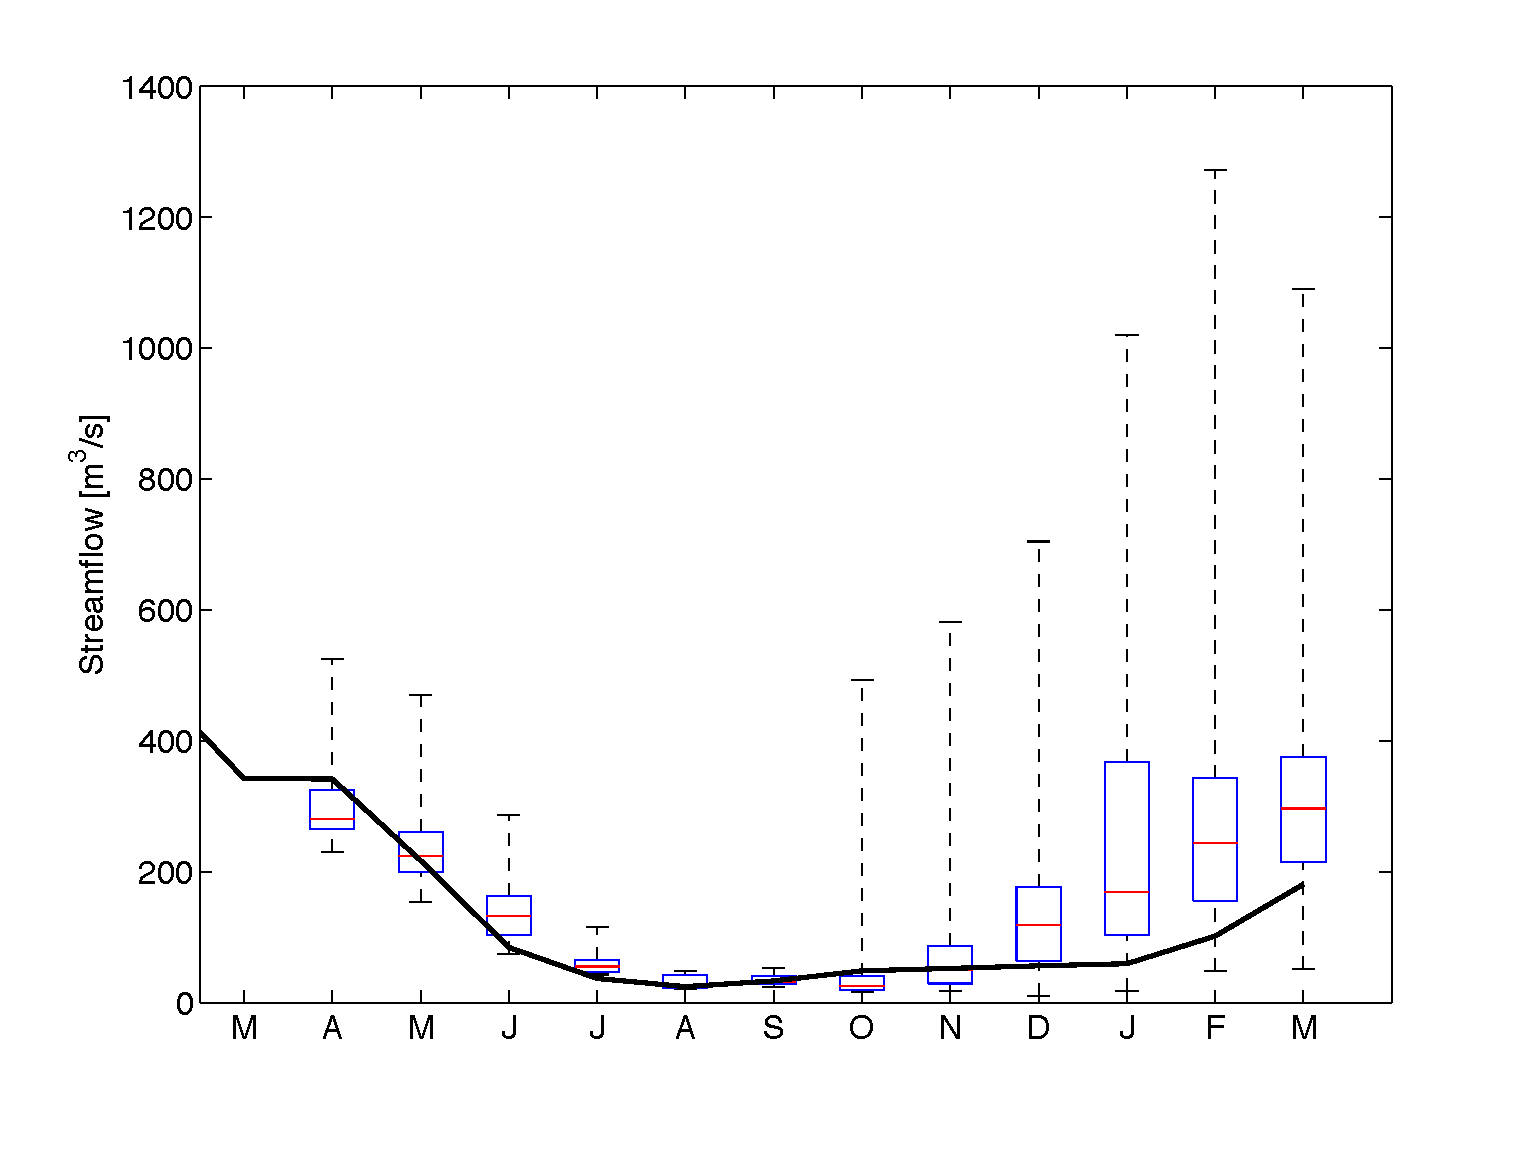
\includegraphics[width=\columnwidth]{Images/Introduction_Writing/boxplot_ensemble_2000.pdf} 
\caption[Streamflow forecast ensemble on April 1st 2000]{Streamflow forecast ensemble on April 1st 2000. The boxes show the 25\%, 50\%, and 75\% percentiles, while the whiskers represent the minimum and maximum ensemble members, thus indicating the full range of uncertainty. The solid black line represents the observations.}
\label{fig:boxplot_quality}
\end{figure}

Figures should always be good quality figures.
Axis tag, labels, and legend should have an appropriate font size.
Keep always the original figure (for example, \verb!.fig! if you created the figure with matlab): this will allow you or who is working with/after you to quickly modify it or recover the original data, if needed.
When applicable, keep the same axis ranges to the figures: it will ease the comparison between different figures.
When applicable/possible, use subfigures to ease the comparison between figures.

Finally, if you are using figures, tables and/or data from other sources, for example from other publications, cite always the reference. 
For example: \\
\blockquote{[...], taken/modified from Jones et al. (1950)}

\section{Mathematics}
Inline vs full line vs numbered equation.
Punctuation within equations.

Contemporary writers label the mathematical results in their papers as lemmas, theorems, propositions and so on.
Typically the major results of the paper are called theorems, the lesser results are called propositions.
The propositions are typically ingredients in the proofs of the theorems that are stand-alone statements of may be of independent interest), and the small technical results are called lemmas.
This probably varies quite a bit from writer to writer (and perhaps also from field to field).

\section{Margin notes}
Margin notes are used to study a new text or paper.
To read carefully a given text, it is essential that you write "all over" what you read, usually in the margins or between the lines?wherever there is space.
By annotating, you'll be creating a shorthand version of what you're reading to which you can return later for reference.
It's always much easier to navigate something you read a few days ago if you have taken detailed marginal notes.
We recommend to use margin notes when reviewing you own thesis.
Marginal notes help you to conceptualize the piece as you read.

Here are some general tips for annotating non-fiction articles.
Right next to each paragraph, write a brief phrase summarizing what happens in it. 
Underline passages that seem crucial to the point of the paragraph or to the larger thesis of the piece.
Note sections you don't fully understand with a question, like "What does this mean?" or "Doesn't this contradict my earlier argument?".
Outline points being made and the examples given to support them.
If you lists a number of reasons or factors that cause something or says something can be divided up into a certain number of parts, list the parts or factors in the margin.

\section{Submission to university: follow the instructions}
Visit \href{http://www.tedoc.polimi.it/tesilaurea/Consegna-tesi-di-laurea-(vecchio-ordinamento-e-specialistica)}{this link} for the updated information about the content of the thesis.

\enquote{Alcune Scuole forniscono linee guida specifiche cui i laureandi devono attenersi per la redazione della tesi. Per ulteriori informazioni:
\href{http://www.tedoc.polimi.it/download/lauree_magistrali/201406_POLITesi_Info_specifiche_scuole.pdf}{www.tedoc.polimi.it/\ldots}}

\subsection{Archiving electronic documents: PDF/A}
PDF/A is an ISO-standardized version of the Portable Document Format (PDF) specialized for the digital preservation of electronic documents. PDF/A differs from PDF by prohibiting features ill-suited to long-term archiving, such as font linking (as opposed to font embedding). The ISO requirements for PDF/A file viewers include color management guidelines, support for embedded fonts, and a user interface for reading embedded annotations.

Universities usually requires this standard but they're also not aware that common programs like MS Word, OpenOffice and so on aren't really able to produce compliant PDFs. In Latex, there's some development going on but at the time of writing, the available commands are still too obscure and buggy. So in the end, forget the PDF/A for now.\footnote{Or DIY and then make a pull request on github :D.}

	\chapter{Practical guide to \enquote{ClassicThesis at DEIB}}
\label{chap:conclusion}
This template is ready to be used when writing a thesis at \myDepartment.
It is a modified version of Classic Thesis by Andr\'e Miede that can be found here \url{http://code.google.com/p/classicthesis/}.

\section{Learn \LaTeX}
\LaTeX\ is a document preparation system and document markup language.
It is widely used for the communication and publication of scientific documents in many fields, including mathematics, physics, computer science, statistics, economics, and political science.

\LaTeX\ users are weird people who care about the ligature between \enquote{f} and \enquote{i} and gets pissed off every time they look at a MS Word document.
Nevertheless, they can explain themselves very well as shown in some beautiful guides for the \LaTeX\ world.
Our preferred one for beginners is \enquote{The Not So Short Introduction to \LaTeXe}, which can be found \href{http://www.ctan.org/pkg/lshort}{here}.\footnote{\url{http://www.ctan.org/pkg/lshort}}
For italians we also strongly suggest \enquote{L'arte di scrivere con \LaTeX}, that can be found \href{http://www.lorenzopantieri.net/LaTeX_files/ArteLaTeX.pdf}{here}.\footnote{\url{http://www.lorenzopantieri.net/LaTeX_files/ArteLaTeX.pdf}}
It contains everything needed, however I suggest the reading of chapter 3 for a short introduction. \enquote{ClassicThesis} is another guide of the same author that can be useful, download it \href{http://www.lorenzopantieri.net/LaTeX_files/ClassicThesis.pdf}{here}.\footnote{\url{http://www.lorenzopantieri.net/LaTeX_files/ClassicThesis.pdf}}

\section{Install \LaTeX}
If you don't have already a \LaTeX\ system installed, this section will explain everything you need.
The easiest way to get \LaTeX\ is to install TeXLive, which works on all \acp{OS}.
In \url{https://www.tug.org/texlive/} you find the instructions and the files needed - and also get in touch with minimalism of \TeX users. 

Then you will need an editor: I strongly recommend TeXworks because it's very simple and available on all the platforms.
Also you don't need to install it, it's already included in TeXLive.
The official documentation of TeXworks is available \href{https://docs.google.com/file/d/0B5iVT8Q7W44pMk1WSFRKcDRlMU0/preview}{here};\footnote{\url{https://docs.google.com/file/d/0B5iVT8Q7W44pMk1WSFRKcDRlMU0/preview}}
I strongly recommend the reading of chapter 3.
Alternatevely you can read an italian manual: \href{http://profs.sci.univr.it/~gregorio/introtexworks.pdf}{profs.sci.univr.it/\ldots} (just 13 pages, read it!).\footnote{If you already have a preferred editor, just keep using yours.}

After opening TeXworks, I strongly suggest to set these two additional things:
\begin{itemize}
	\item open Preferences, then go the Composition tab: in the second box there, the \enquote{Process instruments}, push the plus button.
	In the window just opened, write \verb!Biber! in the \enquote{Name} field, \verb!biber! in the \enquote{Program} field (lowercase!) and then press the plus button to add the argument \verb!$basename!;
	\item again in the same window, set \enquote{Hide console output} to \enquote{never}.
\end{itemize}

Then just test the installation of the template:
\begin{aenumerate}
	\item go into the template home folder;
	\item open the file \verb!ClassicThesis_DEIB.tex!;
	\item select \verb!pdfLaTeX! from the dropdown menu in the top right of the TeXworks window;
	\item press the rounded green button: it compiles the \verb!.tex! file for the first time and open the resulting \verb!.pdf!;
	\item select \verb!Biber! from the same dropdown menu and press again the green button: this compiles the bibliography, a thing you need to repeat only when you change the file \verb!Bibliography.bib!;
	\item select \verb!pdfLaTeX! again and recompile: this is needed to build indices and crossreferences;
\end{aenumerate}
The above compilation procedure is the standard way to translate the \LaTeX\ code into pdfs.

\section{Online editor}
If the above procedure seems too difficult to you and you have an internet connection always available, you might think to use an online editor. The best choice at the time of writing is \url{http:\\\\sharelatex.com} where you can even find this template after registration to the site by looking for \enquote{Classic Thesis At DEIB}. Your project will be saved on their server but you can also download them. The platform allows up to two authors for free accounts.

There is no need to provide instructions for its use since the website has them. They also have an online \LaTeX guide which is also very useful.

\section{Building blocks}

\subsection{File structure}
The template is organized in multiple file and folders:
\begin{aenumerate}

	\item \verb!ClassicThesis_DEIB.tex! is the main file to be compiled, found in the root folder.
You should just add the source filenames you want to include and any hyphenation you need to explictly specify. 

	\item \verb!classicthesis-config.tex! contains options that can be chosen for this template, like the \verb!draft! one that prints date and time at the bottom of every page.
It contains also the definition for the title, the author and others stuff displayed in the titlepage.
Comments within the file should guide you.\footnote{comments are the rows starting with $\%$.} Take a look at it!

	\item \verb!Bibliography.bib! is the \emph{Bibtex} database: it is a normal textfile where you should put books and articles read;

	\item \verb!Chapters! contains the files for the main chapters of your thesis; this is where you will add the chapters text, as well these very words in line 41 of the file \verb!Conclusion.tex!;

	\item \verb!CodeFiles! contains any code snippet you want to include in your thesis with the environment \verb!listings!; it might be some relevant Matlab or C code, as well as long bash scripts;

	\item \verb!FrontBackmatter! contains various files that are included in the main one to produce abstract, titlepages, acknowledgements, \ldots. 
Follow the instructions below to modify them in order to suits your needs;

	\item \verb!Images! contains the \verb!.pdf! or \verb!.png! versions of the images of the thesis.
A \verb!sources! subfolder is also provided for keeping things well organized.

\end{aenumerate}

To modify abstract, preface, acknowledgements snd acronyms, you need to go into the folder \verb!FrontBackmatter! where you will find the following:
\begin{description}

	\item[Abstract.tex] contains the text displayed as \enquote{abstract} and \enquote{sommario} just after the list of figures, tables, etc. Modify the text and leave the rest.

	\item[Acknowledgments.tex] contains the text put just before the table of contents. Modify the text to suit your needs.

	\item[Acronyms.tex] contains the environment \verb!acronym! with the definition of all the acronyms that will be used within the text. Add your own to the list and put the longest as parameter of the environment.
 
	\item[AutoParts] folder contains things that should work without your intervention. Forget them. 

	\item[Dedication.tex] same usage and structure as \verb!Acknowledgements.tex!.

	\item[Estratto.tex] Politecnico di Milano requires an italian long excerpt of theses written in foreign languages.

	\item[Frontespizio.tex] and \verb!FrontespizioIT.tex! are the cover page in english and italian, respectively. Politecnico di Milano requires the italian version of the english cover, so there it is. Both should work perfectly if you modify section 2 of the file \verb!classicthesis-config.tex!, but you may not like the style so modify them as you prefer.
	
	\item[Preface.tex] same usage and structure as \verb!Acknowledgements.tex!.

	\item[Publication.tex] same usage and structure as \verb!Acknowledgements.tex!, but not included by default. Activate it by uncommenting the relevant line in \verb!ClassicThesis_DEIB.tex!.

	\item[RetroFrontespizio.tex] contains the colophon. In most cases is fine as it already is.
\end{description}

\subsection{Special environments}\label{subsec:special_env}
In addition to common \LaTeX\ environments, this thesis is set to use:
\begin{itemize}

	\graffito{The command graffito is used to put some text here, usefull to underline important things before long paragraphs.}

	\item \verb!\begin{aenumerate}! to produce an \verb!\enumerate! with letters instead of numbers, as in the file list above;

	\item \verb!\blockcquote[][]{}{}! to \blockcquote[see][p. 111]{bringhurst:2002}{produce a quotation with reference to author and page}.
	If the quotation is longer than two rows is indented. This is provided by the package \verb!csquotes!, which settings are in \verb!classicthesis-config.tex!. 
	The package also provides \verb!\enquote{!the citation\verb!}! that produces \enquote{correct quatation style} according to the language in use.

	\item \verb!\ac{}! and its variations, defined by package \verb!acronyms!, provide nice handling for acronyms, like \ac{XML}, produced with the code \verb!\ac{XML}!.
	List them within the environment \verb!acronym! in the file \verb!FrontBackmatter/Acronyms.tex!.

	\item the so called semi-dynamic referencing for chapter, sections, subsections, appendices, figures, tables and equations.
	They are a set of commands like \verb!\myChap{label_key}! that produce things like \myChap{chap:aChapter}.
	There are also capital versions of the commands (\verb!\MyChap{}! produces \MyChap{chap:aChapter}).
	They need a \verb!\label{name}! anchor next to the referred thing.
	\begin{itemize}
		\item\verb!\myChap! for chapters;
		\item\verb!\mySec! for sections;
		\item\verb!\mySubsec! for subsections;
		\item\verb!\myAppendix! for appendices;
		\item\verb!\myFig! for figures;
		\item\verb!\myTab! for tables;
		\item\verb!\myEq! for equations;
	\end{itemize}

	\item references to bibliography are produced in the usual way with \verb!\cite{bib_key}! \cite{bringhurst:2002} and its variations \verb!\citeauthor{bib_key}!, \verb!\citetitle{bib_key}! and others.

	\item footnotes are useful to provide information which are not required to understand a sentence but provide interesting details. You can create them with \verb!\footnote{text}!.\footnote{They should be placed after the punctuation mark and preferably at the end of the paragraph. In fact, they should not interrupt the reading flow. If you need to put a footnote in the middle of a paragraph, or of a sentence then the note should be part of the main text.}

	\item figures are handled usually with the code
	\begin{verbatim}
	\begin{figure}
	\centering
	\includegraphics[width=\columnwidth]{Images/your_image_name.pdf} 
	\caption[Short description]{Long description.}
	\label{fig:a_name}
	\end{figure}
	\end{verbatim}
	which produces things like \myFig{fig:massConstraintFeasibility}. 
	Take care of the short description: it appears in the list of figures and should be just a reference, not a exhaustive description.
	Of course, you need to put the image file \verb!your_image_name.pdf! in folder \verb!Images/!.
	We suggest to keep things organized: create a folder for each chapter and keep the original source/working file in the same place.

	\item tables are produced with
	\begin{verbatim}
	\begin{table}[tb]
	\footnotesize
	\centering
	\begin{tabularx}{0.8\textwidth}{llrcl}
	\toprule
	\tableheadline{l}{Algorithm} &
	\tableheadline{l}{Parameter} &
	\tableheadlineMore{3}{c}{Suggested Values} \\
	\midrule
	\tablefirstcol{l}{Any}
	& \acs{NFE} 		& $10\,000 $ & $ \div $ & $ 200\,000$ \\
	& Population Size 	&  $10 $ & $ \div 	$ & $ 1000$ \\
	\midrule
	\tablefirstcol{l}{\ac{GDE3}}
	& \ac{DE} step size & $0.0 $ & $\div $ & $ 1.0$ \\
	& Crossover rate 	& $0.0$ & $ \div $ & $ 1.0$ \\
	\bottomrule
	\end{tabularx}
	\caption[Short description]{Long description.}
	\label{tab:MOEAandParameters}
	\end{table}
	\end{verbatim}
	which produces \myTab{tab:MOEAandParameters}.
	\verb!\myfloatalign!, \verb!\tableheadline{}{}! and its variation \verb!\tableheadlineMore{}{}{}! and \verb!\tablefirstcol{}{}! are used to give a common style to all tables in the document.
	Use them!
	They are defined in \verb!classicthesis-config.tex!.

	\item equation are produced in classic \LaTeX\ way and they turn out be something like this
	\begin{equation}
	\nabla \mathbf{q_s} = U(x,y) - b_t
	\label{eq:massConservation}
	\end{equation}

\end{itemize}

\begin{figure}
\centering
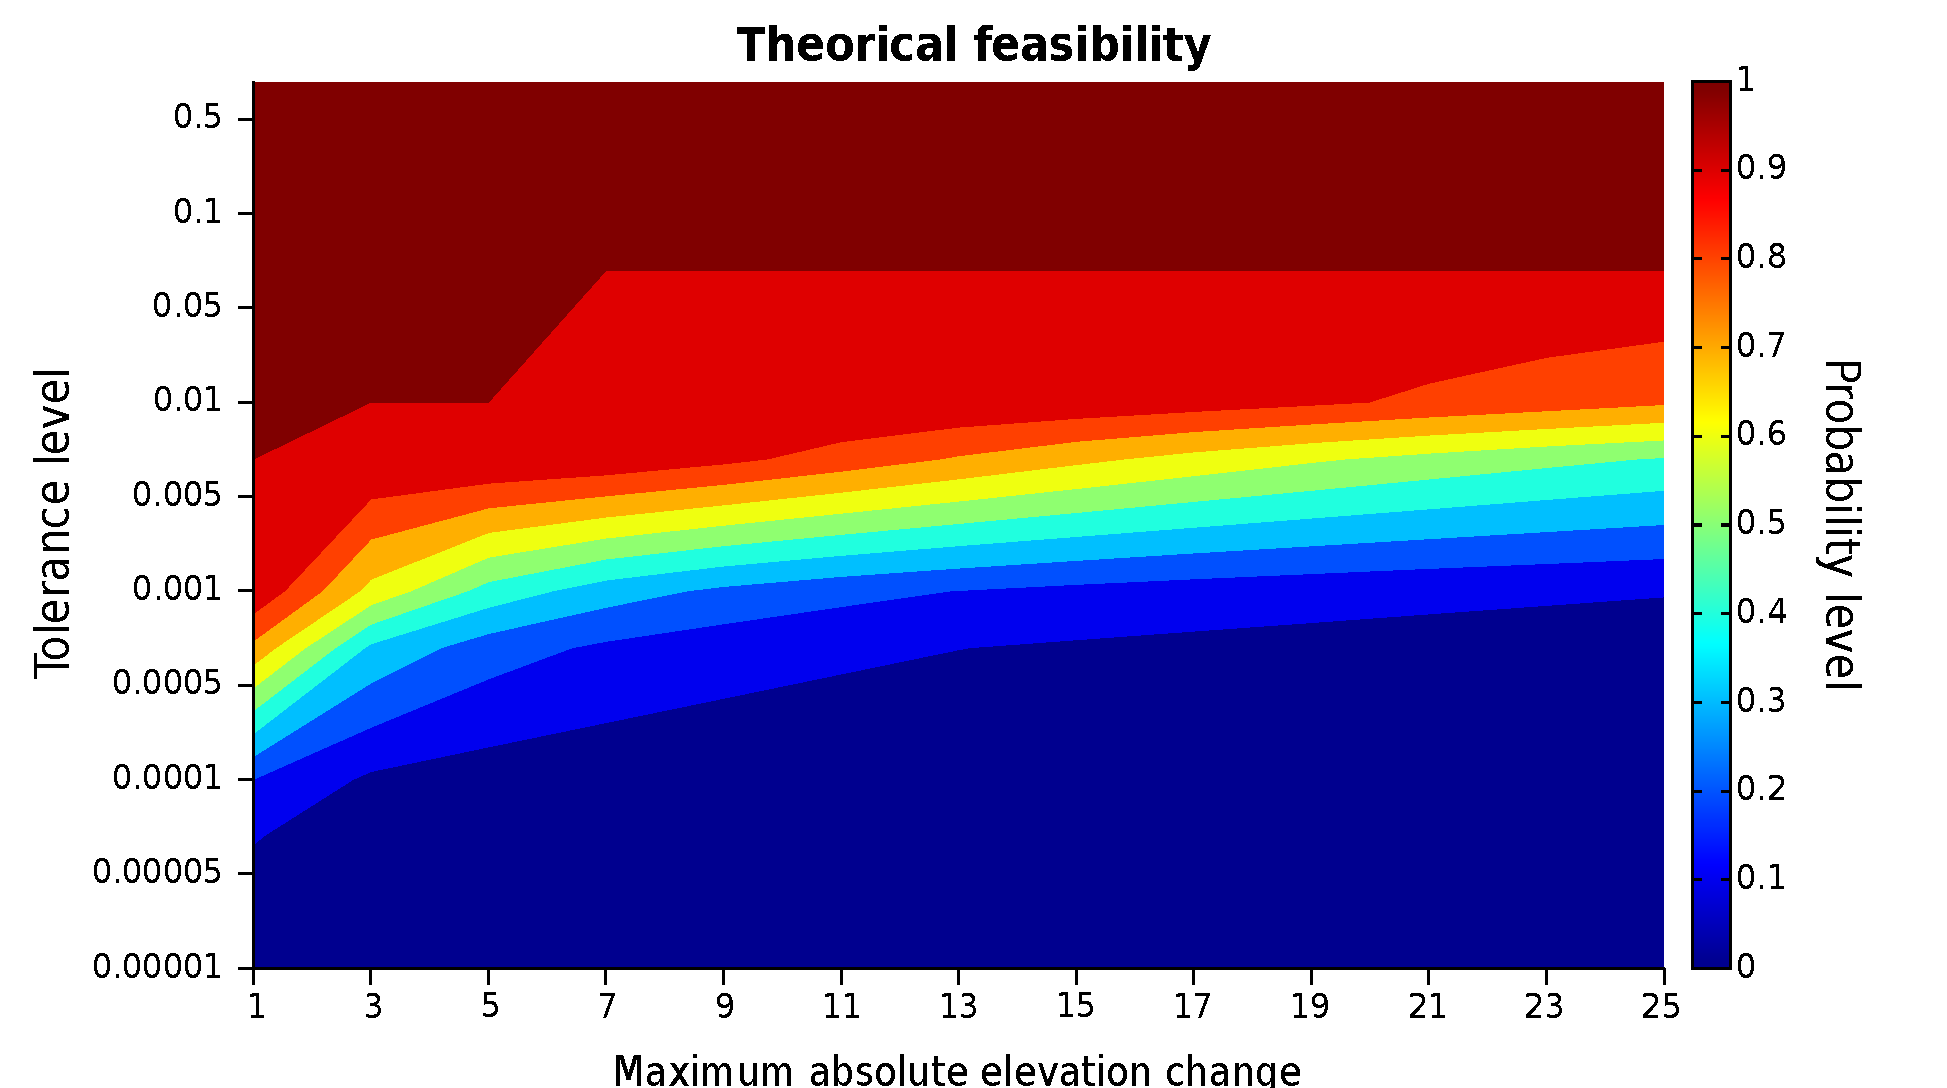
\includegraphics[width=\columnwidth]{Images/Technicalities/feasibilityNR51.pdf}  
\caption[Thing taken from our master thesis]{Thing taken from our master thesis whose meaning have been completely forgotten.}
\label{fig:massConstraintFeasibility}
\end{figure}

\begin{table}
\footnotesize
\centering
\begin{tabularx}{0.8\textwidth}{llrcl}
\toprule
\tableheadline{l}{Algorithm} &
\tableheadline{l}{Parameter} &
\tableheadlineMore{3}{c}{Suggested Values} \\
\midrule
\tablefirstcol{l}{Any}	& NFE	 		& $10\,000 $ 	& $ \div $ 	& $ 200\,000$ \\
				& Population Size 	&  $10 $ 		& $ \div $ 	& $ 1000$ \\
\midrule
\tablefirstcol{l}{GDE3} & DE step size 		& $0.0 $ 	& $\div $ 	& $ 1.0$ \\
				& Crossover rate 	& $0.0$ 	& $ \div $ 	& $ 1.0$ \\
\bottomrule
\end{tabularx}
\caption[Parameters needed for things]{Parameters needed for things that are not needed anymore themselves.}
\label{tab:MOEAandParameters}
\end{table}

\section{Contributing to this template}
Suggestion and improvements are welcome at \url{https://github.com/Lordmzn/ClassicThesis-at-DEIB} or via email at \url{emanuele.mason@polimi.it}, \url{andrea.cominola@polimi.it} or \url{daniela.anghileri@polimi.it}.
 
	
	% ************************************************************
	% Backmatter
	%*************************************************************
	\cleardoublepage%********************************************************************
% Bibliography
%*******************************************************
% work-around to have small caps also here in the headline
\manualmark
\markboth{\spacedlowsmallcaps{\bibname}}{\spacedlowsmallcaps{\bibname}}
%\phantomsection 
\refstepcounter{dummy} 
% to have the bib a bit from the rest in the toc
\addtocontents{toc}{\protect\vspace{\beforebibskip}}
\addcontentsline{toc}{chapter}{\tocEntry{\bibname}}
\label{app:bibliography} 
\printbibliography
	\appendix
	% \cleardoublepage\part{Appendix}
	%********************************************************************
% Appendix
%*******************************************************
% If problems with the headers: get headings in appendix etc. right
\markboth{\spacedlowsmallcaps{Appendix}}{\spacedlowsmallcaps{Appendix}}
%************************************************
\chapter{Appendix example: code listings}

\begin{flushright}{\slshape    
    We have seen that computer programming is an art, \\ 
    because it applies accumulated knowledge to the world, \\ 
    because it requires skill and ingenuity, and especially \\
    because it produces objects of beauty.} \\ \medskip
    --- \citeauthor{knuth:1974}, \citetitle{knuth:1974},
\citeyear{knuth:1974} 
\end{flushright}

\section{The \texttt{listings} package to include source code}
Source code is usually not part of the text of a thesis, but if it is an original contribution it makes sense to le the code speak by itself instead of describing it. The package \verb!listings! provide the proper layout tools. Refer to its manual if you need to use it, an example is given in listing \ref{lst:probCounter}.

\lstinputlisting[
	firstline=1,
	lastline=47,
	float=tb,
	language=C++,
	tabsize=2,
	numbers=left,
	numberstyle=\tiny,
	stepnumber=2,
	numbersep=5pt,
	caption={Code snippet with the recursive function to evaluate the pdf of the sum $Z_N$ of $N$ random variables equal to $X$.}, 
	captionpos=t,
	label=lst:probCounter
	]{CodeFiles/probabilityCounter.cpp}

\end{document}
% ****************************************************************